%=======================================================================
%  CH 4 — NUMERICAL PROBLEMS & SOLUTIONS
%=======================================================================
\section*{\color{acc}Ch 4 --- Association Analysis --- Numerical Problems \& Solutions}
\vspace{-4pt}{\color{acc}\rule{\textwidth}{1.1pt}}\vspace{4pt}

{\color{sub}\footnotesize 5 methods $\cdot$ 14 PYQ instances $\cdot$ every itemset count recomputed
from the printed transaction tables. \mk{This is the heaviest numerical chapter in the syllabus.}}

\lead{Methods}
\begin{itemize}
  \item \textbf{M1} Apriori: candidate generation, pruning, frequent itemsets
  \item \textbf{M2} Rule generation from frequent itemsets
  \item \textbf{M3} FP-tree construction and FP-Growth mining
  \item \textbf{M4} Pattern evaluation: lift and the correlation measures
  \item \textbf{M5} Subsequence enumeration
\end{itemize}

\begin{center}\fbox{\begin{minipage}{0.92\textwidth}\small
\mk{Convert the threshold to a COUNT before you start.} ``min support 50\%'' on 6 transactions
means a count of 3. Nearly every lost mark in this chapter comes from mixing percentages and counts
half way through. Write \emph{min\_sup\_count $=$ N} at the top and use only that. \\
Also: \mk{support is over ALL transactions; confidence is over the antecedent's transactions only.}
\end{minipage}}\end{center}

\hr

%=======================================================================
\T{M1. Apriori}

\lead{Method}
\begin{enumerate}
  \item Scan once, count items $\rightarrow$ keep those $\ge$ min\_sup\_count $\rightarrow$ $L_1$.
  \item \textbf{Join} $L_{k-1}$ with itself: combine 2 itemsets only if their first $k-2$ items match.
  \item \textbf{Prune}: discard a candidate if \emph{any} of its $(k-1)$-subsets is missing from $L_{k-1}$.
  \item \textbf{Count} survivors against $D$, keep those meeting the threshold $\rightarrow$ $L_k$.
  \item Stop when $L_k$ is empty.
\end{enumerate}
\begin{itemize}
  \item \mk{Show the prune step explicitly} --- it is where the method marks are.
\end{itemize}

\creamq{Problem 1.1}{\m{2+7}}
\begin{asked}{2080 Bhadra \textperiodcentered{} Q3 (b) \textperiodcentered{} [2+7]}
What is Association Analysis? Explain with different use cases? Use the Apriori algorithm to
find the frequent itemsets. Assume minimum support count is 4 and confidence is 80\%.
\par\vspace{2pt}
\par
\begin{tabularx}{0.62\textwidth}{@{}L{1.9cm}X@{}}
\toprule
\hrow \thead{TID} & \thead{Items} \\
T100 & F, A, C, D, G, I, M, P, N \\
T101 & A, B, C, D, F, L, M, O, P \\
T102 & B, F, H, V, J, O, P \\
T103 & B, C, K, S, A, V \\
T104 & L, A, F, C, E, P, M, N, V \\
T105 & I, B, A, P, S, M \\
T106 & F, A, C, I, B, A, P \\
\bottomrule
\end{tabularx}
\end{asked}
{\color{sub}\footnotesize T106 genuinely prints ``F, A, C, I, B, A, P'' ---
\mk{A is repeated; a transaction is a set}, so treat it as \{F,A,C,I,B,P\}.}

\lead{Step 1: $C_1 \rightarrow L_1$} \; count all 18 distinct items over the 7 transactions,
min count $=4$
\par
\begin{tabularx}{\textwidth}{@{}L{0.9cm}L{1.0cm}L{0.9cm}@{\hspace{10pt}}L{0.9cm}L{1.0cm}L{0.9cm}@{\hspace{10pt}}L{0.9cm}L{1.0cm}L{0.9cm}@{\hspace{10pt}}L{0.9cm}L{1.0cm}X@{}}
\toprule
\hrow \thead{It.} & \thead{Cnt} & \thead{Keep} & \thead{It.} & \thead{Cnt} & \thead{Keep} &
      \thead{It.} & \thead{Cnt} & \thead{Keep} & \thead{It.} & \thead{Cnt} & \thead{Keep} \\
\midrule
A & 6 & \checkmark & F & 5 & \checkmark & K & 1 & \xmark & O & 2 & \xmark \\
B & 5 & \checkmark & G & 1 & \xmark      & L & 2 & \xmark & P & 6 & \checkmark \\
C & 5 & \checkmark & H & 1 & \xmark      & M & 4 & \checkmark & S & 2 & \xmark \\
D & 2 & \xmark     & I & 3 & \xmark      & N & 2 & \xmark & V & 3 & \xmark \\
E & 1 & \xmark     & J & 1 & \xmark      &   &   &        &   &   &  \\
\bottomrule
\end{tabularx}
\par\penalty0\vspace{1pt}
$\mathbf{L_1 = \{A(6),\ B(5),\ C(5),\ F(5),\ M(4),\ P(6)\}}$ \; --- 6 items survive of 18.

\penalty0\vspace{3pt}
\lead{Step 2: $C_2 \rightarrow L_2$} \; all $\binom{6}{2} = 15$ pairs from $L_1$, counted against $D$
\par
\begin{tabularx}{\textwidth}{@{}L{1.2cm}L{1.0cm}L{0.9cm}@{\hspace{10pt}}L{1.2cm}L{1.0cm}L{0.9cm}@{\hspace{10pt}}L{1.2cm}L{1.0cm}L{0.9cm}@{\hspace{10pt}}L{1.2cm}L{1.0cm}X@{}}
\toprule
\hrow \thead{Pair} & \thead{Cnt} & \thead{Keep} & \thead{Pair} & \thead{Cnt} & \thead{Keep} &
      \thead{Pair} & \thead{Cnt} & \thead{Keep} & \thead{Pair} & \thead{Cnt} & \thead{Keep} \\
\midrule
AB & 4 & \checkmark & AP & 5 & \checkmark & BP & 4 & \checkmark & CP & 4 & \checkmark \\
AC & 5 & \checkmark & BC & 3 & \xmark     & CF & 4 & \checkmark & FM & 3 & \xmark \\
AF & 4 & \checkmark & BF & 3 & \xmark     & CM & 3 & \xmark     & FP & 5 & \checkmark \\
AM & 4 & \checkmark & BM & 2 & \xmark     &    &   &            & MP & 4 & \checkmark \\
\bottomrule
\end{tabularx}
\par\penalty0\vspace{1pt}
$\mathbf{L_2 = \{AB(4),\ AC(5),\ AF(4),\ AM(4),\ AP(5),\ BP(4),\ CF(4),\ CP(4),\ FP(5),\ MP(4)\}}$

\penalty0\vspace{3pt}
\lead{Step 3: $C_3 \rightarrow L_3$} \; join $L_2$ pairs sharing their first item, then
\mk{prune before counting}
\par
\begin{tabularx}{\textwidth}{@{}L{1.5cm}X L{3.2cm}L{1.1cm}L{0.9cm}@{}}
\toprule
\hrow \thead{Cand.} & \thead{Subset test (all 2-subsets must be in $L_2$)} & \thead{Transactions}
& \thead{Count} & \thead{Keep} \\
\midrule
ABC & BC $\notin L_2$ & \mk{pruned, never counted} & --- & \xmark \\
ABF & BF $\notin L_2$ & \mk{pruned, never counted} & --- & \xmark \\
ABM & BM $\notin L_2$ & \mk{pruned, never counted} & --- & \xmark \\
ABP & AB \checkmark\ AP \checkmark\ BP \checkmark\ $\rightarrow$ survives pruning
    & T101, T105, T106 & 3 & \xmark \\
ACF & AC \checkmark\ AF \checkmark\ CF \checkmark & T100, T101, T104, T106 & 4 & \checkmark \\
ACM & CM $\notin L_2$ & \mk{pruned, never counted} & --- & \xmark \\
ACP & AC \checkmark\ AP \checkmark\ CP \checkmark & T100, T101, T104, T106 & 4 & \checkmark \\
AFM & FM $\notin L_2$ & \mk{pruned, never counted} & --- & \xmark \\
AFP & AF \checkmark\ AP \checkmark\ FP \checkmark & T100, T101, T104, T106 & 4 & \checkmark \\
AMP & AM \checkmark\ AP \checkmark\ MP \checkmark & T100, T101, T104, T105 & 4 & \checkmark \\
CFP & CF \checkmark\ CP \checkmark\ FP \checkmark & T100, T101, T104, T106 & 4 & \checkmark \\
\bottomrule
\end{tabularx}
\par\penalty0\vspace{1pt}
$\mathbf{L_3 = \{ACF(4),\ ACP(4),\ AFP(4),\ AMP(4),\ CFP(4)\}}$
\begin{itemize}
  \item \mk{Five candidates died at the prune step without a single database scan} --- that saving
        is the whole point of the Apriori property, so show the column.
  \item ABP is the instructive one: it \emph{passes} pruning and still fails on the count.
        \mk{Pruning is sufficient to reject, never sufficient to accept.}
\end{itemize}

\penalty0\vspace{2pt}
\lead{Step 4: $C_4 \rightarrow L_4$} \; join $L_3$ triples sharing their first \emph{two} items
\par
\begin{tabularx}{\textwidth}{@{}L{1.5cm}L{3.0cm}X L{1.1cm}L{0.9cm}@{}}
\toprule
\hrow \thead{Cand.} & \thead{Joined from} & \thead{Subset test} & \thead{Count} & \thead{Keep} \\
\midrule
ACFP & ACF $+$ ACP & ACF \checkmark\ ACP \checkmark\ AFP \checkmark\ CFP \checkmark &
       4 \; \footnotesize (T100, T101, T104, T106) & \checkmark \\
\bottomrule
\end{tabularx}
\par\penalty0\vspace{1pt}
$\mathbf{L_4 = \{ACFP(4)\}}$; \; no two 4-itemsets remain to join $\rightarrow$ $C_5 = \emptyset$
$\rightarrow$ \textbf{stop}.

\lead{Frequent itemsets} Maximal frequent itemset $=$ \mk{\textbf{\{A, C, F, P\}} with support
4/7 $=$ 57\%}.
\begin{itemize}
  \item \textbf{Check}: all $2^4-2 = 14$ proper subsets of ACFP do appear in $L_1$--$L_3$ above. \checkmark
\end{itemize}

\lead{Step 5: the rules \mk{(the question gives confidence $=$ 80\,\%, so this half is asked)}}
\begin{itemize}
  \item From the maximal itemset $l = \{A,C,F,P\}$, $\sigma(l) = 4$. For every non-empty proper
        subset $s$, output $s \Rightarrow (l-s)$ with
        $conf = \dfrac{\sigma(l)}{\sigma(s)} = \dfrac{4}{\sigma(s)}$.
  \item $2^4 - 2 = \mathbf{14}$ candidate rules. \mk{$conf \ge 0.80$ needs $\sigma(s) \le 5$}, so
        read the answer straight off the antecedent's count.
\end{itemize}

\sbsr{0.52}{%
\par
\begin{tabularx}{\linewidth}{@{}L{2.5cm}L{1.0cm}X@{}}
\toprule
\hrow \thead{Rule} & \thead{$\sigma(s)$} & \thead{Confidence} \\
\midrule
$C \Rightarrow AFP$   & 5 & $4/5 = 80\,\%$ \checkmark \\
$F \Rightarrow ACP$   & 5 & $4/5 = 80\,\%$ \checkmark \\
$AC \Rightarrow FP$   & 5 & $4/5 = 80\,\%$ \checkmark \\
$AP \Rightarrow CF$   & 5 & $4/5 = 80\,\%$ \checkmark \\
$FP \Rightarrow AC$   & 5 & $4/5 = 80\,\%$ \checkmark \\
$AF \Rightarrow CP$   & 4 & $4/4 = 100\,\%$ \checkmark \\
$CF \Rightarrow AP$   & 4 & $4/4 = 100\,\%$ \checkmark \\
$CP \Rightarrow AF$   & 4 & $4/4 = 100\,\%$ \checkmark \\
$ACF \Rightarrow P$   & 4 & $4/4 = 100\,\%$ \checkmark \\
$ACP \Rightarrow F$   & 4 & $4/4 = 100\,\%$ \checkmark \\
$AFP \Rightarrow C$   & 4 & $4/4 = 100\,\%$ \checkmark \\
$CFP \Rightarrow A$   & 4 & $4/4 = 100\,\%$ \checkmark \\
\midrule
$A \Rightarrow CFP$   & 6 & $4/6 = 66.7\,\%$ \xmark \\
$P \Rightarrow ACF$   & 6 & $4/6 = 66.7\,\%$ \xmark \\
\bottomrule
\end{tabularx}}{%
\lead{Reading the table}
\begin{itemize}
  \item \mk{\textbf{12 of the 14 rules are strong}} at min\_conf $=$ 80\,\%.
  \item The only two failures are the ones with $A$ or $P$ \emph{alone} on the left. Both occur in
        6 of the 7 transactions, so they are \mk{too common to predict anything}: a frequent
        antecedent divides the confidence down.
  \item \mk{The general lesson}: confidence falls as the antecedent gets more frequent, and rises
        as it gets more specific. Longer left-hand sides almost always score higher.
  \item Seven rules here sit at \textbf{100\,\%}. By \S4.1 those are the \emph{least} interesting
        of the twelve, because $\{A,F\}$ never appears without $C$ and $P$ anywhere in this
        database $\rightarrow$ nothing actionable. \mk{Say so if the question asks you to
        comment}, do not just report the highest number.
\end{itemize}}

\creamq{Problem 1.2}{\m{5}}
\begin{asked}{2080 Baishakh \textperiodcentered{} Q5 \textperiodcentered{} [4+5]}
Generally, we will be more interested in associated rules with high confidence. However, often
we will not be interested in association rules that have a confidence of 100\%. Why? Then
specifically explain why association rules with 99\% confidence may be interesting (i.e., what
might they indicate)? Identify the candidate and large item sets of the following transaction
table using Apriori algorithm with minimum support 2.
\par\vspace{2pt}
\par
\begin{tabularx}{0.42\textwidth}{@{}L{1.9cm}X@{}}
\toprule
\hrow \thead{TID} & \thead{Items} \\
10 & A, C, D \\
20 & B, C, E \\
30 & A, B, C, E \\
40 & B, E \\
\bottomrule
\end{tabularx}
\end{asked}

\sbsr{0.46}{%
\lead{Step 1: $C_1 \rightarrow L_1$} \; min count $=2$
\par
\begin{tabularx}{\linewidth}{@{}L{1.1cm}X L{1.0cm}L{0.9cm}@{}}
\toprule
\hrow \thead{Item} & \thead{In} & \thead{Count} & \thead{Keep} \\
\midrule
A & 10, 30     & 2 & \checkmark \\
B & 20, 30, 40 & 3 & \checkmark \\
C & 10, 20, 30 & 3 & \checkmark \\
D & 10         & 1 & \xmark \\
E & 20, 30, 40 & 3 & \checkmark \\
\bottomrule
\end{tabularx}
\par\penalty0\vspace{1pt}
$\mathbf{L_1 = \{A(2),\ B(3),\ C(3),\ E(3)\}}$}{%
\lead{Step 2: $C_2 \rightarrow L_2$} \; all $\binom{4}{2} = 6$ pairs from $L_1$
\par
\begin{tabularx}{\linewidth}{@{}L{1.3cm}X L{1.0cm}L{0.9cm}@{}}
\toprule
\hrow \thead{Pair} & \thead{In} & \thead{Count} & \thead{Keep} \\
\midrule
AB & 30         & 1 & \xmark \\
AC & 10, 30     & 2 & \checkmark \\
AE & 30         & 1 & \xmark \\
BC & 20, 30     & 2 & \checkmark \\
BE & 20, 30, 40 & 3 & \checkmark \\
CE & 20, 30     & 2 & \checkmark \\
\bottomrule
\end{tabularx}
\par\penalty0\vspace{1pt}
$\mathbf{L_2 = \{AC(2),\ BC(2),\ BE(3),\ CE(2)\}}$}

\penalty0\vspace{3pt}
\lead{Step 3: $C_3 \rightarrow L_3$} \; join $L_2$ on a shared first item, prune, then count
\par
\begin{tabularx}{\textwidth}{@{}L{1.8cm}L{3.5cm}X L{1.7cm}L{1.0cm}L{0.9cm}@{}}
\toprule
\hrow \thead{Joined from} & \thead{Candidate} & \thead{Subset test} & \thead{In} & \thead{Count}
& \thead{Keep} \\
\midrule
BC $+$ BE & \textbf{BCE} & BC \checkmark\ BE \checkmark\ CE \checkmark\ $\rightarrow$ survives
          & 20, 30 & 2 & \checkmark \\
AC $+$ --- & none & AC is the only pair starting with A, so it has nothing to join with
          & --- & --- & --- \\
\bottomrule
\end{tabularx}
\par\penalty0\vspace{1pt}
$\mathbf{L_3 = \{BCE(2)\}}$; \; $C_4$ needs two 3-itemsets sharing a prefix and there is only
one $\rightarrow$ \textbf{stop}.

\lead{Final answer} Frequent itemsets: A, B, C, E, AC, BC, BE, CE, BCE.

\creamq{Problem 1.3}{\m{10}}
\begin{asked}{2070 Chaitra \textperiodcentered{} Q4 \textperiodcentered{} [10]}
Explain Apriori algorithm. Use Apriori to generate frequent item sets with support of 50\% for
the following transaction database.
\par\vspace{2pt}
\par
\begin{tabularx}{0.36\textwidth}{@{}L{1.9cm}X@{}}
\toprule
\hrow \thead{TID} & \thead{Items} \\
1 & ACD \\
2 & BD \\
3 & ABCE \\
4 & BDF \\
\bottomrule
\end{tabularx}
\end{asked}
{\color{sub}\footnotesize 4 transactions, 50\% $\rightarrow$ min count $=$ 2.}
\begin{itemize}
  \item $L_1$: A(2), B(3), C(2), D(3) \quad (E:1, F:1 dropped)
  \item $C_2$: AB(1)\xmark AC(2)\checkmark AD(1)\xmark BC(1)\xmark BD(2)\checkmark CD(1)\xmark
  \item $\mathbf{L_2 = \{AC(2),\ BD(2)\}}$
  \item $C_3$: AC and BD share no common prefix $\rightarrow$ \textbf{no candidates}. Stop.
\end{itemize}
\lead{Final answer} Frequent itemsets: A, B, C, D, AC, BD.

\creamq{Problems 1.4 and 1.5}{\m{5+3}\m{8}}
\begin{asked}{2076 Chaitra \textperiodcentered{} Q7 \textperiodcentered{} [5+3]}
Consider the transaction data shown in the following table from a fast food restaurant.
\par\vspace{2pt}
\par
\begin{tabularx}{0.62\textwidth}{@{}L{2.3cm}X@{}}
\toprule
\hrow \thead{Meal Item} & \thead{List of Item IDs} \\
Order:1 & M1, M2, M5 \\
Order:2 & M2, M4 \\
Order:3 & M2, M3 \\
Order:4 & M1, M2, M4 \\
Order:5 & M1, M3 \\
Order:6 & M2, M3 \\
Order:7 & M1, M3 \\
Order:8 & M1, M2, M3, M5 \\
Order:9 & M1, M2, M3 \\
\bottomrule
\end{tabularx}
\par\vspace{2pt}
There are 9 distinct transactions (Order:~1 -- Order:~9) and each transaction involves between
2 and 4 meal items. There are a total of 5 meal items that are involved in the transactions.
For simplicity, the meal items have been assigned short names (M1--M5). Assume that the minimum
support is 2/9 and the minimum confidence is 7/9.
\begin{enumerate}[label=\alph*), leftmargin=1.6em]
  \item Apply the Apriori algorithm to the dataset of transactions and identify all frequent
        $k$-itemsets.
  \item Find all strong association rules of the form: $X \wedge Y \rightarrow Z$ and note
        their confidence values.
\end{enumerate}
\end{asked}
\begin{asked}{2074 Ashwin \textperiodcentered{} Q5 \textperiodcentered{} [8]}
Identify the candidate, frequent item sets and association rules for the following transaction
data using Apriori algorithm.
\par\vspace{2pt}
\par
\begin{tabularx}{0.50\textwidth}{@{}L{1.9cm}X@{}}
\toprule
\hrow \thead{TID} & \thead{ITEMS} \\
1 & M1, M2, M5 \\
2 & M2, M4 \\
3 & M2, M3 \\
4 & M1, M2, M4 \\
5 & M1, M3 \\
6 & M2, M3 \\
7 & M1, M3 \\
8 & M1, M2, M3, M5 \\
9 & M1, M2, M3 \\
\bottomrule
\end{tabularx}
\par\vspace{2pt}
Take minimum support $=$ 20\%, minimum confidence 80\%
\end{asked}
{\color{sub}\footnotesize \mk{Identical 9-transaction table, and both thresholds work out to a
count of 2}, so the frequent itemsets are the same; only the rule filter differs.}

\lead{Frequent itemsets} (9 transactions, min count 2)

\sbsr{0.42}{%
\lead{Step 1: $C_1 \rightarrow L_1$}
\par
\begin{tabularx}{\linewidth}{@{}L{1.1cm}X L{1.0cm}L{0.9cm}@{}}
\toprule
\hrow \thead{Item} & \thead{In} & \thead{Count} & \thead{Keep} \\
\midrule
M1 & T1,4,5,7,8,9   & 6 & \checkmark \\
M2 & T1,2,3,4,6,8,9 & 7 & \checkmark \\
M3 & T3,5,6,7,8,9   & 6 & \checkmark \\
M4 & T2,4           & 2 & \checkmark \\
M5 & T1,8           & 2 & \checkmark \\
\bottomrule
\end{tabularx}
\par\penalty0\vspace{1pt}
\mk{Nothing is dropped} --- all 5 items clear a count of 2.}{%
\lead{Step 2: $C_2 \rightarrow L_2$} \; all $\binom{5}{2} = 10$ pairs
\par
\begin{tabularx}{\linewidth}{@{}L{1.4cm}X L{1.0cm}L{0.9cm}@{}}
\toprule
\hrow \thead{Pair} & \thead{In} & \thead{Count} & \thead{Keep} \\
\midrule
M1M2 & T1, T4, T8, T9 & 4 & \checkmark \\
M1M3 & T5, T7, T8, T9 & 4 & \checkmark \\
M1M4 & T4             & 1 & \xmark \\
M1M5 & T1, T8         & 2 & \checkmark \\
M2M3 & T3, T6, T8, T9 & 4 & \checkmark \\
M2M4 & T2, T4         & 2 & \checkmark \\
M2M5 & T1, T8         & 2 & \checkmark \\
M3M4 & ---            & 0 & \xmark \\
M3M5 & T8             & 1 & \xmark \\
M4M5 & ---            & 0 & \xmark \\
\bottomrule
\end{tabularx}}

\penalty0\vspace{2pt}
$\mathbf{L_2}$ $=$ \{$\mathbf{M1M2(4)}$, $\mathbf{M1M3(4)}$, $\mathbf{M1M5(2)}$,
$\mathbf{M2M3(4)}$, $\mathbf{M2M4(2)}$, $\mathbf{M2M5(2)}$\}

\penalty0\vspace{3pt}
\lead{Step 3: $C_3 \rightarrow L_3$} \; join two $L_2$ pairs \mk{only when both are in $L_2$ and
they share their first item}
\par
\begin{tabularx}{\textwidth}{@{}L{2.6cm}L{1.9cm}X L{1.5cm}L{1.0cm}L{0.9cm}@{}}
\toprule
\hrow \thead{Joined from} & \thead{Candidate} & \thead{Subset test} & \thead{In} & \thead{Count}
& \thead{Keep} \\
\midrule
M1M2 $+$ M1M3 & M1M2M3 & M1M2 \checkmark\ M1M3 \checkmark\ M2M3 \checkmark & T8, T9 & 2 & \checkmark \\
M1M2 $+$ M1M5 & M1M2M5 & M1M2 \checkmark\ M1M5 \checkmark\ M2M5 \checkmark & T1, T8 & 2 & \checkmark \\
M1M3 $+$ M1M5 & M1M3M5 & M3M5 $\notin L_2$ $\rightarrow$ \mk{pruned} & --- & --- & \xmark \\
M2M3 $+$ M2M4 & M2M3M4 & M3M4 $\notin L_2$ $\rightarrow$ \mk{pruned} & --- & --- & \xmark \\
M2M3 $+$ M2M5 & M2M3M5 & M3M5 $\notin L_2$ $\rightarrow$ \mk{pruned} & --- & --- & \xmark \\
M2M4 $+$ M2M5 & M2M4M5 & M4M5 $\notin L_2$ $\rightarrow$ \mk{pruned} & --- & --- & \xmark \\
\bottomrule
\end{tabularx}
\par\penalty0\vspace{1pt}
$\mathbf{L_3 = \{M1M2M3(2),\ M1M2M5(2)\}}$
\begin{itemize}
  \item \mk{Note what is \emph{not} in the table}: M1M2M4 never appears, because generating it
        would need M1M4, and M1M4 failed at step 2. \mk{A candidate is only ever built from two
        surviving parents} --- it is not built and then pruned.
\end{itemize}

\penalty0\vspace{2pt}
\lead{Step 4: $C_4 \rightarrow L_4$}
\par
\begin{tabularx}{\textwidth}{@{}L{2.4cm}L{1.8cm}X L{1.0cm}L{0.85cm}@{}}
\toprule
\hrow \thead{Joined from} & \thead{Candidate} & \thead{Subset test} & \thead{Count} & \thead{Keep} \\
\midrule
M1M2M3 $+$ M1M2M5 & M1M2M3M5 & M1M3M5 $\notin L_3$ $\rightarrow$ \mk{pruned} & --- & \xmark \\
\bottomrule
\end{tabularx}
\par\penalty0\vspace{1pt}
$L_4 = \emptyset$ $\rightarrow$ \textbf{stop}.

\penalty0\vspace{2pt}
\lead{The one idea that decides every rule below}
\begin{itemize}
  \item Every rule out of an itemset $l$ has the \emph{same} numerator:
        $conf(s \Rightarrow l-s) = \sigma(l)/\sigma(s)$. \mk{Only the antecedent's count moves.}
  \item So a rule is strong exactly when \mk{the antecedent is nearly as rare as the whole
        itemset} $\rightarrow$ when the antecedent hardly ever appears without the consequent.
  \item Here $\sigma(\text{M4}) = \sigma(\text{M5}) = 2$, and both \emph{always} appear with their
        partners. \mk{Expect every strong rule to have M4 or M5 on the left}, and check that
        prediction against the tables. Nothing else can win, because M1, M2 and M3 each occur
        6--7 times while no itemset containing them has support above 4.
\end{itemize}

\penalty0\vspace{2pt}
\lead{1.4 \; Rules of the form $X \wedge Y \Rightarrow Z$, \; min conf $= 7/9 = 0.778$}
\begin{itemize}
  \item That form means a \textbf{2-item antecedent and a 1-item consequent}, so only the
        \textbf{3-itemsets} in $L_3$ can produce one. Two of them, three rules each
        $\rightarrow$ \mk{6 candidates, and they are all of them}.
\end{itemize}

\sbsr{0.56}{%
\par
\begin{tabularx}{\linewidth}{@{}L{2.2cm}L{2.7cm}L{0.85cm}X@{}}
\toprule
\hrow \thead{From} & \thead{Rule} & \thead{$\sigma(XY)$} & \thead{Conf $= 2/\sigma(XY)$} \\
\midrule
M1M2M3 & M1$\wedge$M2$\Rightarrow$M3 & 4 & $0.50$ \xmark \\
$\sigma = 2$ & M1$\wedge$M3$\Rightarrow$M2 & 4 & $0.50$ \xmark \\
       & M2$\wedge$M3$\Rightarrow$M1 & 4 & $0.50$ \xmark \\
\addlinespace[2pt]
M1M2M5 & M1$\wedge$M2$\Rightarrow$M5 & 4 & $0.50$ \xmark \\
$\sigma = 2$ & \textbf{M1$\wedge$M5$\Rightarrow$M2} & 2 & $\mathbf{1.00}$ \checkmark \\
       & \textbf{M2$\wedge$M5$\Rightarrow$M1} & 2 & $\mathbf{1.00}$ \checkmark \\
\bottomrule
\end{tabularx}}{%
\lead{Answer to 1.4}
\begin{itemize}
  \item \mk{\textbf{2 strong rules}, both at 100\,\% confidence}:
        M1$\wedge$M5$\Rightarrow$M2 and M2$\wedge$M5$\Rightarrow$M1.
  \item Every rule out of M1M2M3 fails, and all three fail \emph{identically} at $0.50$, because
        all three of its 2-subsets happen to have $\sigma = 4$.
  \item The two winners are exactly the ones predicted above: \mk{M5 is in the antecedent}, and
        M5 occurs only in T1 and T8, both of which also hold M1 and M2.
\end{itemize}}

\penalty0\vspace{3pt}
\lead{1.5 \; \emph{All} association rules, \; min conf $= 0.80$}
\begin{itemize}
  \item Now every frequent itemset with $|l| \ge 2$ contributes: six 2-itemsets ($2$ rules each)
        and two 3-itemsets ($2^3 - 2 = 6$ rules each) $\rightarrow$ \mk{$12 + 12 = 24$ candidate
        rules}. All 24 are listed, none is skipped.
\end{itemize}

\par
\begin{tabularx}{\textwidth}{@{}L{1.9cm}L{2.8cm}L{0.75cm}L{1.45cm}@{\hspace{4pt}}L{1.9cm}L{2.8cm}L{0.75cm}X@{}}
\toprule
\hrow \thead{From} & \thead{Rule} & \thead{$\sigma(s)$} & \thead{Conf} &
\thead{From} & \thead{Rule} & \thead{$\sigma(s)$} & \thead{Conf} \\
\midrule
M1M2 $(4)$ & M1$\Rightarrow$M2 & 6 & $0.67$ \xmark &
M2M5 $(2)$ & M2$\Rightarrow$M5 & 7 & $0.29$ \xmark \\
           & M2$\Rightarrow$M1 & 7 & $0.57$ \xmark &
           & \textbf{M5$\Rightarrow$M2} & 2 & $\mathbf{1.00}$ \checkmark \\
\addlinespace[2pt]
M1M3 $(4)$ & M1$\Rightarrow$M3 & 6 & $0.67$ \xmark &
M1M2M3 $(2)$ & M1$\Rightarrow$M2M3 & 6 & $0.33$ \xmark \\
           & M3$\Rightarrow$M1 & 6 & $0.67$ \xmark &
           & M2$\Rightarrow$M1M3 & 7 & $0.29$ \xmark \\
\addlinespace[2pt]
M1M5 $(2)$ & M1$\Rightarrow$M5 & 6 & $0.33$ \xmark &
           & M3$\Rightarrow$M1M2 & 6 & $0.33$ \xmark \\
           & \textbf{M5$\Rightarrow$M1} & 2 & $\mathbf{1.00}$ \checkmark &
           & M1$\wedge$M2$\Rightarrow$M3 & 4 & $0.50$ \xmark \\
\addlinespace[2pt]
M2M3 $(4)$ & M2$\Rightarrow$M3 & 7 & $0.57$ \xmark &
           & M1$\wedge$M3$\Rightarrow$M2 & 4 & $0.50$ \xmark \\
           & M3$\Rightarrow$M2 & 6 & $0.67$ \xmark &
           & M2$\wedge$M3$\Rightarrow$M1 & 4 & $0.50$ \xmark \\
\addlinespace[2pt]
M2M4 $(2)$ & M2$\Rightarrow$M4 & 7 & $0.29$ \xmark &
M1M2M5 $(2)$ & M1$\Rightarrow$M2M5 & 6 & $0.33$ \xmark \\
           & \textbf{M4$\Rightarrow$M2} & 2 & $\mathbf{1.00}$ \checkmark &
           & M2$\Rightarrow$M1M5 & 7 & $0.29$ \xmark \\
\addlinespace[2pt]
           &  &  &  &
           & \textbf{M5$\Rightarrow$M1$\wedge$M2} & 2 & $\mathbf{1.00}$ \checkmark \\
           &  &  &  &
           & M1$\wedge$M2$\Rightarrow$M5 & 4 & $0.50$ \xmark \\
           &  &  &  &
           & \textbf{M1$\wedge$M5$\Rightarrow$M2} & 2 & $\mathbf{1.00}$ \checkmark \\
           &  &  &  &
           & \textbf{M2$\wedge$M5$\Rightarrow$M1} & 2 & $\mathbf{1.00}$ \checkmark \\
\bottomrule
\end{tabularx}

\lead{Answer to 1.5}
\begin{itemize}
  \item \mk{\textbf{6 strong rules}, every one of them at 100\,\% confidence}:
  \begin{itemize}
    \item[] M5$\Rightarrow$M1 \quad M5$\Rightarrow$M2 \quad M4$\Rightarrow$M2 \quad
            M5$\Rightarrow$M1$\wedge$M2 \quad M1$\wedge$M5$\Rightarrow$M2 \quad
            M2$\wedge$M5$\Rightarrow$M1
  \end{itemize}
  \item The other 18 fail, and \mk{the prediction held}: every survivor has M4 or M5 on the left.
        M1, M2 and M3 are too frequent to be confident antecedents here, the best any of them
        manages is $0.67$.
  \item \textbf{Cross-check with 1.4}: the two rules found there must reappear here, since 1.4's
        threshold ($0.778$) is the tighter of the two. They do, on the last two rows. \checkmark
  \item \mk{Worth a closing sentence}: all six sit at 100\,\%, which by \S4.1 makes them
        \emph{reliable but not surprising} $\rightarrow$ M4 and M5 are simply never ordered
        alone. Confidence alone cannot see that; lift would.
\end{itemize}

\creamq{Problem 1.6}{\m{8}}
\begin{asked}{2079 Bhadra \textperiodcentered{} Q5 \textperiodcentered{} [8]}
Derive association rule for the following market basket transactions.

Minimum support $=$ 50\% \qquad Minimum confidence $=$ 80\%
\par\vspace{2pt}
\par
\begin{tabularx}{0.46\textwidth}{@{}L{3.0cm}X@{}}
\toprule
\hrow \thead{Transaction ID} & \thead{Item Set} \\
1 & A,B \\
2 & A,D \\
3 & A,C \\
4 & B,E \\
5 & B,D,E \\
6 & A,E,C \\
\bottomrule
\end{tabularx}
\end{asked}
{\color{sub}\footnotesize \mk{This one has a surprise.} \gap 6 transactions,
50\,\% $\rightarrow$ min count $= 3$.}

\sbs{%
\lead{Step 1: $C_1 \rightarrow L_1$}
\par
\begin{tabularx}{\linewidth}{@{}L{1.0cm}X L{1.0cm}L{0.9cm}@{}}
\toprule
\hrow \thead{Item} & \thead{In} & \thead{Count} & \thead{Keep} \\
\midrule
A & 1, 2, 3, 6 & 4 & \checkmark \\
B & 1, 4, 5    & 3 & \checkmark \\
C & 3, 6       & 2 & \xmark \\
D & 2, 5       & 2 & \xmark \\
E & 4, 5, 6    & 3 & \checkmark \\
\bottomrule
\end{tabularx}
\par\penalty0\vspace{1pt}
$\mathbf{L_1 = \{A(4),\ B(3),\ E(3)\}}$}{%
\lead{Step 2: $C_2 \rightarrow L_2$} \; the 3 pairs from $L_1$
\par
\begin{tabularx}{\linewidth}{@{}L{1.0cm}X L{1.0cm}L{0.9cm}@{}}
\toprule
\hrow \thead{Pair} & \thead{In} & \thead{Count} & \thead{Keep} \\
\midrule
AB & 1     & 1 & \xmark \\
AE & 6     & 1 & \xmark \\
BE & 4, 5  & 2 & \xmark \\
\bottomrule
\end{tabularx}
\par\penalty0\vspace{1pt}
$\mathbf{L_2 = \emptyset}$ \; --- every pair falls short.}

\lead{Final answer}
\begin{itemize}
  \item \mk{No frequent 2-itemset exists, so \textbf{no association rule can be derived} at
        50\,\% support.} Say this explicitly --- it is the correct answer, not a dead end.
  \item And it holds \mk{for every confidence threshold, including 0\,\%}: a rule needs a
        2-itemset to split, and there is none. \mk{Lowering min\_conf cannot rescue it, only
        lowering min\_sup can} (\S4.2).
  \item \textbf{Show you understand why}: the data is spread thin, every pair occurs at most twice.
  \item \textbf{If min support is relaxed to 33.3\,\%} (count 2), the picture changes:
\end{itemize}

\par
\begin{tabularx}{\textwidth}{@{}L{1.5cm}L{1.1cm}L{2.5cm}L{1.5cm}X@{}}
\toprule
\hrow \thead{New $L_2$} & \thead{Count} & \thead{Rule} & \thead{Confidence} & \thead{Strong at 80\,\%?} \\
\midrule
AC & 2 & A $\Rightarrow$ C & $2/4 = 0.50$ & \xmark \\
   &   & \textbf{C $\Rightarrow$ A} & $\mathbf{2/2 = 1.00}$ & \checkmark \\
\addlinespace[2pt]
BE & 2 & B $\Rightarrow$ E & $2/3 = 0.67$ & \xmark \\
   &   & E $\Rightarrow$ B & $2/3 = 0.67$ & \xmark \\
\bottomrule
\end{tabularx}
\par\penalty0\vspace{1pt}
\mk{One rule survives}: \textbf{C $\Rightarrow$ A} at 100\,\%. Worth adding as a closing
remark. \added

\creamq{Problem 1.7}{\m{2+8}}
\begin{asked}{2082 Bhadra \textperiodcentered{} Q4 \textperiodcentered{} [2+8]}
Explain the term support and confidence in association analysis. Derive association rule for
following transaction considering minimum support $=$ 60\% and confidence $=$ 80\% using Apriori
Algorithm.
\par\penalty0\vspace{2pt}
\par
\begin{tabularx}{0.52\textwidth}{@{}L{1.6cm}X@{}}
\toprule
\hrow \thead{TID} & \thead{Transaction} \\
T1 & A, B, C, D, E, F \\
T2 & B, C, D, E, F, G \\
T3 & A, D, E, H \\
T4 & A, D, F, I, J \\
T5 & B, D, E, K \\
\bottomrule
\end{tabularx}
\end{asked}
{\color{sub}\footnotesize 5 transactions, 60\,\% $\rightarrow$ \mk{min count $= 3$}.}

\sbs{%
\lead{Step 1: $C_1 \rightarrow L_1$} \; 11 distinct items
\par
\begin{tabularx}{\linewidth}{@{}L{1.0cm}XL{1.0cm}L{0.9cm}@{}}
\toprule
\hrow \thead{Item} & \thead{In} & \thead{Cnt} & \thead{Keep} \\
\midrule
A & T1, T3, T4     & 3 & \checkmark \\
B & T1, T2, T5     & 3 & \checkmark \\
C & T1, T2         & 2 & \xmark \\
D & T1--T5         & 5 & \checkmark \\
E & T1, T2, T3, T5 & 4 & \checkmark \\
F & T1, T2, T4     & 3 & \checkmark \\
G & T2             & 1 & \xmark \\
H & T3             & 1 & \xmark \\
I & T4             & 1 & \xmark \\
J & T4             & 1 & \xmark \\
K & T5             & 1 & \xmark \\
\bottomrule
\end{tabularx}
\par\penalty0\vspace{1pt}
$\mathbf{L_1 = \{A(3), B(3), D(5), E(4), F(3)\}}$}{%
\lead{Step 2: $C_2 \rightarrow L_2$} \; all $\binom{5}{2} = 10$ pairs
\par
\begin{tabularx}{\linewidth}{@{}L{1.2cm}XL{1.0cm}L{0.9cm}@{}}
\toprule
\hrow \thead{Pair} & \thead{In} & \thead{Cnt} & \thead{Keep} \\
\midrule
AB & T1             & 1 & \xmark \\
AD & T1, T3, T4     & 3 & \checkmark \\
AE & T1, T3         & 2 & \xmark \\
AF & T1, T4         & 2 & \xmark \\
BD & T1, T2, T5     & 3 & \checkmark \\
BE & T1, T2, T5     & 3 & \checkmark \\
BF & T1, T2         & 2 & \xmark \\
DE & T1, T2, T3, T5 & 4 & \checkmark \\
DF & T1, T2, T4     & 3 & \checkmark \\
EF & T1, T2         & 2 & \xmark \\
\bottomrule
\end{tabularx}
\par\penalty0\vspace{1pt}
$\mathbf{L_2 = \{AD(3), BD(3), BE(3), DE(4), DF(3)\}}$}

\penalty0\vspace{3pt}
\lead{Step 3: $C_3 \rightarrow L_3$}
\par
\begin{tabularx}{\textwidth}{@{}L{2.2cm}L{1.6cm}X L{2.2cm}L{1.0cm}L{0.9cm}@{}}
\toprule
\hrow \thead{Joined from} & \thead{Cand.} & \thead{Subset test} & \thead{In} & \thead{Cnt}
& \thead{Keep} \\
\midrule
BD $+$ BE & \textbf{BDE} & BD \checkmark\ BE \checkmark\ DE \checkmark & T1, T2, T5 & 3 & \checkmark \\
AD $+$ --- & none & AD is the only pair starting with A & --- & --- & --- \\
DE $+$ DF & DEF & EF $\notin L_2$ $\rightarrow$ \mk{pruned} & --- & --- & \xmark \\
\bottomrule
\end{tabularx}
\par\penalty0\vspace{1pt}
$\mathbf{L_3 = \{BDE(3)\}}$; \; $C_4 = \emptyset$ $\rightarrow$ \textbf{stop}.

\lead{Step 4: the rules} \; $5 \times 2 + (2^3-2) = \mathbf{16}$ candidates, min conf 80\,\%
\par
\begin{tabularx}{\textwidth}{@{}L{1.8cm}L{2.6cm}L{0.9cm}L{1.7cm}@{\hspace{6pt}}L{1.8cm}L{2.6cm}L{0.9cm}X@{}}
\toprule
\hrow \thead{From} & \thead{Rule} & \thead{$\sigma(s)$} & \thead{Conf} &
      \thead{From} & \thead{Rule} & \thead{$\sigma(s)$} & \thead{Conf} \\
\midrule
AD $(3)$ & \textbf{A $\Rightarrow$ D} & 3 & $\mathbf{1.00}$ \checkmark &
DF $(3)$ & D $\Rightarrow$ F & 5 & $0.60$ \xmark \\
         & D $\Rightarrow$ A & 5 & $0.60$ \xmark &
         & \textbf{F $\Rightarrow$ D} & 3 & $\mathbf{1.00}$ \checkmark \\
\addlinespace[2pt]
BD $(3)$ & \textbf{B $\Rightarrow$ D} & 3 & $\mathbf{1.00}$ \checkmark &
BDE $(3)$ & \textbf{B $\Rightarrow$ DE} & 3 & $\mathbf{1.00}$ \checkmark \\
         & D $\Rightarrow$ B & 5 & $0.60$ \xmark &
          & D $\Rightarrow$ BE & 5 & $0.60$ \xmark \\
\addlinespace[2pt]
BE $(3)$ & \textbf{B $\Rightarrow$ E} & 3 & $\mathbf{1.00}$ \checkmark &
          & E $\Rightarrow$ BD & 4 & $0.75$ \xmark \\
         & E $\Rightarrow$ B & 4 & $0.75$ \xmark &
          & \textbf{BD $\Rightarrow$ E} & 3 & $\mathbf{1.00}$ \checkmark \\
\addlinespace[2pt]
DE $(4)$ & \textbf{D $\Rightarrow$ E} & 5 & $\mathbf{0.80}$ \checkmark &
          & \textbf{BE $\Rightarrow$ D} & 3 & $\mathbf{1.00}$ \checkmark \\
         & \textbf{E $\Rightarrow$ D} & 4 & $\mathbf{1.00}$ \checkmark &
          & DE $\Rightarrow$ B & 4 & $0.75$ \xmark \\
\bottomrule
\end{tabularx}
\begin{itemize}
  \item \mk{\textbf{9 strong rules} of 16.} $D \Rightarrow E$ scrapes in at exactly $0.80$
        --- \mk{$\ge$ the threshold counts as passing}, so keep it.
  \item Every failure has $D$ or $E$ alone on the left. $D$ is in \emph{all five} transactions,
        so it predicts nothing (\S4.1); it is the consequent of four winning rules instead.
\end{itemize}

\creamq{Problem 1.8}{\m{2+6}}
\begin{asked}{2081 Bhadra \textperiodcentered{} Q7 \textperiodcentered{} [2+6]}
For the transaction given below, consider Confidence $=$ 65\% and minimum support $=$ 50\%.
Identify frequent itemsets with possible association rules using Apriori Algorithm.
\par\penalty0\vspace{2pt}
\par
\begin{tabularx}{0.56\textwidth}{@{}L{1.3cm}X@{}}
\toprule
\hrow \thead{TID} & \thead{Items} \\
1 & MILK, BREAD, CAKE \\
2 & BUTTER, BREAD, EGG \\
3 & MILK, BUTTER, BREAD, EGG \\
4 & BUTTER, EGG \\
\bottomrule
\end{tabularx}
\end{asked}
{\color{sub}\footnotesize 4 transactions, 50\,\% $\rightarrow$ \mk{min count $= 2$}.
\gap \mk{Note the unusually low confidence bar}, 65\,\%, which is why almost everything survives.}

\sbs{%
\lead{Step 1: $C_1 \rightarrow L_1$}
\par
\begin{tabularx}{\linewidth}{@{}L{1.7cm}XL{1.0cm}L{0.9cm}@{}}
\toprule
\hrow \thead{Item} & \thead{In} & \thead{Cnt} & \thead{Keep} \\
\midrule
MILK   & 1, 3    & 2 & \checkmark \\
BREAD  & 1, 2, 3 & 3 & \checkmark \\
CAKE   & 1       & 1 & \xmark \\
BUTTER & 2, 3, 4 & 3 & \checkmark \\
EGG    & 2, 3, 4 & 3 & \checkmark \\
\bottomrule
\end{tabularx}
\par\penalty0\vspace{1pt}
$\mathbf{L_1 = \{MILK(2), BREAD(3), BUTTER(3), EGG(3)\}}$}{%
\lead{Step 2: $C_2 \rightarrow L_2$} \; 6 pairs
\par
\begin{tabularx}{\linewidth}{@{}L{2.6cm}XL{1.0cm}L{0.9cm}@{}}
\toprule
\hrow \thead{Pair} & \thead{In} & \thead{Cnt} & \thead{Keep} \\
\midrule
BREAD, BUTTER & 2, 3    & 2 & \checkmark \\
BREAD, EGG    & 2, 3    & 2 & \checkmark \\
BREAD, MILK   & 1, 3    & 2 & \checkmark \\
BUTTER, EGG   & 2, 3, 4 & 3 & \checkmark \\
BUTTER, MILK  & 3       & 1 & \xmark \\
EGG, MILK     & 3       & 1 & \xmark \\
\bottomrule
\end{tabularx}}

\penalty0\vspace{2pt}
\lead{Step 3: $C_3 \rightarrow L_3$}
\par
\begin{tabularx}{\textwidth}{@{}L{4.2cm}L{3.6cm}X L{1.0cm}L{0.9cm}@{}}
\toprule
\hrow \thead{Joined from} & \thead{Candidate} & \thead{Subset test} & \thead{Cnt} & \thead{Keep} \\
\midrule
\{BR,BU\} $+$ \{BR,EG\} & \textbf{BREAD, BUTTER, EGG} &
  all three 2-subsets in $L_2$ \checkmark & 2 & \checkmark \\
\{BR,BU\} $+$ \{BR,MI\} & BREAD, BUTTER, MILK & \{BU,MI\} $\notin L_2$ $\rightarrow$ \mk{pruned}
  & --- & \xmark \\
\{BR,EG\} $+$ \{BR,MI\} & BREAD, EGG, MILK & \{EG,MI\} $\notin L_2$ $\rightarrow$ \mk{pruned}
  & --- & \xmark \\
\bottomrule
\end{tabularx}
\par\penalty0\vspace{1pt}
$\mathbf{L_3 = \{\{BREAD, BUTTER, EGG\}(2)\}}$, \; $C_4 = \emptyset$ $\rightarrow$ stop.

\lead{Step 4: the rules} \; $4 \times 2 + 6 = \mathbf{14}$ candidates, min conf 65\,\%
\par
\begin{tabularx}{\textwidth}{@{}L{4.6cm}L{1.0cm}L{1.7cm}@{\hspace{8pt}}L{4.6cm}L{1.0cm}X@{}}
\toprule
\hrow \thead{Rule} & \thead{$\sigma(s)$} & \thead{Conf} &
      \thead{Rule} & \thead{$\sigma(s)$} & \thead{Conf} \\
\midrule
BREAD $\Rightarrow$ BUTTER & 3 & $0.667$ \checkmark &
BUTTER $\Rightarrow$ EGG   & 3 & $\mathbf{1.00}$ \checkmark \\
BUTTER $\Rightarrow$ BREAD & 3 & $0.667$ \checkmark &
EGG $\Rightarrow$ BUTTER   & 3 & $\mathbf{1.00}$ \checkmark \\
BREAD $\Rightarrow$ EGG    & 3 & $0.667$ \checkmark &
BREAD $\Rightarrow$ BU,EG  & 3 & $0.667$ \checkmark \\
EGG $\Rightarrow$ BREAD    & 3 & $0.667$ \checkmark &
BUTTER $\Rightarrow$ BR,EG & 3 & $0.667$ \checkmark \\
BREAD $\Rightarrow$ MILK   & 3 & $0.667$ \checkmark &
EGG $\Rightarrow$ BR,BU    & 3 & $0.667$ \checkmark \\
MILK $\Rightarrow$ BREAD   & 2 & $\mathbf{1.00}$ \checkmark &
BR,BU $\Rightarrow$ EGG    & 2 & $\mathbf{1.00}$ \checkmark \\
                           &   &                 &
BR,EG $\Rightarrow$ BUTTER & 2 & $\mathbf{1.00}$ \checkmark \\
                           &   &                 &
BU,EG $\Rightarrow$ BREAD  & 3 & $0.667$ \checkmark \\
\bottomrule
\end{tabularx}
\begin{itemize}
  \item \mk{All 14 rules are strong.} That is the point of the 65\,\% threshold: the lowest
        confidence anywhere in this database is $2/3 = 0.667$, which clears it.
  \item \mk{Say so explicitly rather than listing 14 rules and stopping} --- ``every candidate
        rule passes, because min\_conf sits below the minimum achievable confidence here'' is the
        observation worth a mark. Raise the bar to 70\,\% and only the five 100\,\% rules survive.
\end{itemize}

\creamq{Problem 1.9}{\m{3+7}}
\begin{asked}{2073 Chaitra \textperiodcentered{} Q5 \textperiodcentered{} [3+7]}
Explain Apriori algorithm in market basket analysis? Derive association rule from the following
market basket transactions with 50\% of minimum support and confidence respectively.
\par\penalty0\vspace{2pt}
\par
\begin{tabularx}{0.44\textwidth}{@{}L{2.6cm}X@{}}
\toprule
\hrow \thead{Transaction} & \thead{Itemsets} \\
1 & A, B, C \\
2 & A, C \\
3 & A, D \\
4 & B, E, F \\
\bottomrule
\end{tabularx}
\end{asked}
{\color{sub}\footnotesize ``50\,\% of minimum support and confidence respectively'' means
\mk{both} thresholds are 50\,\%: min count $= 2$, min conf $= 0.50$.}

\sbs{%
\lead{Step 1: $C_1 \rightarrow L_1$}
\par
\begin{tabularx}{\linewidth}{@{}L{1.0cm}XL{1.0cm}L{0.9cm}@{}}
\toprule
\hrow \thead{Item} & \thead{In} & \thead{Cnt} & \thead{Keep} \\
\midrule
A & 1, 2, 3 & 3 & \checkmark \\
B & 1, 4    & 2 & \checkmark \\
C & 1, 2    & 2 & \checkmark \\
D & 3       & 1 & \xmark \\
E & 4       & 1 & \xmark \\
F & 4       & 1 & \xmark \\
\bottomrule
\end{tabularx}
\par\penalty0\vspace{1pt}
$\mathbf{L_1 = \{A(3), B(2), C(2)\}}$}{%
\lead{Step 2: $C_2 \rightarrow L_2$}
\par
\begin{tabularx}{\linewidth}{@{}L{1.2cm}XL{1.0cm}L{0.9cm}@{}}
\toprule
\hrow \thead{Pair} & \thead{In} & \thead{Cnt} & \thead{Keep} \\
\midrule
AB & 1    & 1 & \xmark \\
AC & 1, 2 & 2 & \checkmark \\
BC & 1    & 1 & \xmark \\
\bottomrule
\end{tabularx}
\par\penalty0\vspace{1pt}
$\mathbf{L_2 = \{AC(2)\}}$; only one pair survives, so $C_3 = \emptyset$ $\rightarrow$ stop.}

\lead{Step 3: the rules} \; only $\{A,C\}$ can produce any, so $2^2-2 = 2$ candidates
\par
\begin{tabularx}{\textwidth}{@{}L{3.0cm}L{2.0cm}L{3.0cm}X@{}}
\toprule
\hrow \thead{Rule} & \thead{$\sigma(s)$} & \thead{Confidence} & \thead{Strong at 50\,\%?} \\
\midrule
A $\Rightarrow$ C & 3 & $2/3 = 0.667$ & \checkmark \\
C $\Rightarrow$ A & 2 & $2/2 = 1.000$ & \checkmark \\
\bottomrule
\end{tabularx}
\begin{itemize}
  \item \mk{Both are strong}: \textbf{A $\Rightarrow$ C} (67\,\%) and
        \textbf{C $\Rightarrow$ A} (100\,\%).
  \item \mk{Transaction 4 contributes nothing.} $\{B,E,F\}$ shares no item pattern with the rest,
        which is why $B$ survives as a 1-itemset but never appears in a rule. Worth a sentence.
\end{itemize}

\creamq{Problem 1.10}{\m{5+3}}
\begin{asked}{2079 Baishakh \textperiodcentered{} Q5 \textperiodcentered{} [5+3]}
a) Write Apriori algorithm and using the algorithm find all the frequent itemset for the
following database. (min\_sup $=$ 20\%).
\par\penalty0\vspace{2pt}
\par
\begin{tabularx}{0.86\textwidth}{@{}L{1.1cm}L{0.8cm}L{0.8cm}L{0.8cm}L{0.8cm}L{0.8cm}L{0.8cm}L{0.8cm}L{0.8cm}X@{}}
\toprule
\hrow \thead{TID} & \thead{A1} & \thead{A2} & \thead{A3} & \thead{A4} & \thead{A5} & \thead{A6}
 & \thead{A7} & \thead{A8} & \thead{A9} \\
\midrule
T2 & 0 & 1 & 0 & 1 & 0 & 0 & 0 & 1 & 0 \\
T3 & 0 & 0 & 0 & 1 & 1 & 0 & 1 & 0 & 0 \\
T4 & 0 & 0 & 1 & 0 & 0 & 0 & 0 & 0 & 0 \\
T5 & 0 & 0 & 0 & 0 & 1 & 1 & 1 & 0 & 0 \\
T6 & 0 & 1 & 1 & 1 & 0 & 0 & 0 & 0 & 0 \\
T7 & 0 & 1 & 0 & 0 & 0 & 1 & 1 & 0 & 1 \\
T8 & 0 & 0 & 0 & 0 & 1 & 0 & 0 & 0 & 0 \\
\bottomrule
\end{tabularx}
\par\penalty0\vspace{2pt}
b) Is it possible to generate any rules out of the frequent items, considering any value of
confidence threshold?
\end{asked}
{\color{sub}\footnotesize \mk{The table really does start at T2}, has seven rows, and its 8th
column really is headed \texttt{A8} (the scan clips the 8). \gap $20\,\%$ of 7 transactions
$= 1.4$, and a count cannot be fractional, so \mk{min count $= 2$}. \gap
\mk{Column A1 is 0 in every row} --- it can never be frequent, so drop it at once and say why.}

\sbs{%
\lead{(a) Step 1: $C_1 \rightarrow L_1$}
\par
\begin{tabularx}{\linewidth}{@{}L{1.1cm}XL{1.0cm}L{0.9cm}@{}}
\toprule
\hrow \thead{Item} & \thead{In} & \thead{Cnt} & \thead{Keep} \\
\midrule
A1 & --- \mk{(all zero)} & 0 & \xmark \\
A2 & T2, T6, T7 & 3 & \checkmark \\
A3 & T4, T6     & 2 & \checkmark \\
A4 & T2, T3, T6 & 3 & \checkmark \\
A5 & T3, T5, T8 & 3 & \checkmark \\
A6 & T5, T7     & 2 & \checkmark \\
A7 & T3, T5, T7 & 3 & \checkmark \\
A8 & T2         & 1 & \xmark \\
A9 & T7         & 1 & \xmark \\
\bottomrule
\end{tabularx}}{%
\lead{Step 2: $C_2 \rightarrow L_2$} \; $\binom{6}{2} = 15$ pairs
\par
\begin{tabularx}{\linewidth}{@{}L{1.6cm}L{1.0cm}L{0.9cm}@{\hspace{8pt}}L{1.6cm}L{1.0cm}X@{}}
\toprule
\hrow \thead{Pair} & \thead{Cnt} & \thead{Keep} & \thead{Pair} & \thead{Cnt} & \thead{Keep} \\
\midrule
A2,A3 & 1 & \xmark     & A4,A5 & 1 & \xmark \\
A2,A4 & 2 & \checkmark & A4,A6 & 0 & \xmark \\
A2,A5 & 0 & \xmark     & A4,A7 & 1 & \xmark \\
A2,A6 & 1 & \xmark     & A5,A6 & 1 & \xmark \\
A2,A7 & 1 & \xmark     & A5,A7 & 2 & \checkmark \\
A3,A4 & 1 & \xmark     & A6,A7 & 2 & \checkmark \\
A3,A5 & 0 & \xmark     &       &   & \\
A3,A6 & 0 & \xmark     &       &   & \\
A3,A7 & 0 & \xmark     &       &   & \\
\bottomrule
\end{tabularx}}

\penalty0\vspace{2pt}
\lead{Step 3: $C_3$}
\begin{itemize}
  \item $L_2 = \{\text{A2A4}(2),\ \text{A5A7}(2),\ \text{A6A7}(2)\}$.
  \item To build a 3-itemset two pairs must \mk{share their first item}. A2A4, A5A7 and A6A7 all
        start with a different item, so \mk{no candidate can be formed at all}
        $\rightarrow$ $C_3 = \emptyset$ $\rightarrow$ stop.
  \item \textbf{Frequent itemsets}: A2, A3, A4, A5, A6, A7, \{A2,A4\}, \{A5,A7\}, \{A6,A7\}.
\end{itemize}

\lead{(b) Can any rule be generated, at \emph{any} confidence threshold?}
\begin{itemize}
  \item \mk{Yes.} The question is a trap only if you stop at $L_1$: a rule needs a frequent
        itemset of size $\ge 2$ to split into antecedent and consequent, and here \mk{three
        2-itemsets survive}, so rules exist.
  \item Each 2-itemset yields $2^2 - 2 = 2$ rules, so \mk{6 rules in total}:
\end{itemize}
\par
\begin{tabularx}{\textwidth}{@{}L{2.6cm}L{1.2cm}L{2.6cm}X@{}}
\toprule
\hrow \thead{Rule} & \thead{$\sigma(s)$} & \thead{Confidence} & \thead{Comment} \\
\midrule
A2 $\Rightarrow$ A4 & 3 & $2/3 = 0.667$ & \\
A4 $\Rightarrow$ A2 & 3 & $2/3 = 0.667$ & \\
A5 $\Rightarrow$ A7 & 3 & $2/3 = 0.667$ & \\
A7 $\Rightarrow$ A5 & 3 & $2/3 = 0.667$ & \\
A6 $\Rightarrow$ A7 & 2 & $2/2 = 1.000$ & \mk{A6 never occurs without A7} \\
A7 $\Rightarrow$ A6 & 3 & $2/3 = 0.667$ & \\
\bottomrule
\end{tabularx}
\begin{itemize}
  \item So the honest answer is: \mk{rules exist for any threshold up to 0.667}, and above that
        only \textbf{A6 $\Rightarrow$ A7} survives. Above $1.0$ nothing does.
  \item \mk{The general principle} (\S4.2): rules exist iff $L_2 \ne \emptyset$. \textbf{Check
        $L_2$, not the confidence value} --- if $L_2$ were empty no threshold, not even 0\,\%,
        could produce a rule. Compare Problem 1.6, where exactly that happens.
\end{itemize}

\hr

%=======================================================================
\T{M2. Rule generation from frequent itemsets}

\lead{Method}
\begin{itemize}
  \item For each frequent itemset $l$ with $|l| \ge 2$, take every non-empty proper subset $s$:
        \[ s \Rightarrow (l-s) \quad\text{with}\quad
           conf = \frac{sup\_count(l)}{sup\_count(s)} \]
  \item Keep it if $conf \ge$ min\_conf. A $k$-itemset gives $2^k-2$ candidate rules.
  \item \mk{The support of every rule from $l$ is the same} ($= sup(l)$); only confidence varies.
  \item \textbf{Shortcut}: if $s \Rightarrow (l-s)$ fails, every rule whose antecedent is a
        \emph{subset} of $s$ also fails. Prune downward.
\end{itemize}

\creamq{Worked example}{}
\begin{asked}[PROBLEM]{not a PYQ \textperiodcentered{} the rule half of 2081 Baishakh Q3 (b) \added}
The frequent itemset $l = \{$K, E, O$\}$ has support count 3 in the 5-transaction database of
Problem 3.1, where $sup$(K)~$=5$, $sup$(E)~$=4$, $sup$(O)~$=3$, $sup$(K,E)~$=4$,
$sup$(K,O)~$=3$ and $sup$(E,O)~$=3$. List every association rule that $l$ can generate and its
confidence, and say which are strong at a minimum confidence of 80\%.
\end{asked}
From $l=\{$K,E,O$\}$ with $sup=3$ (see Problem 3.1), $|l|=3 \rightarrow 6$ candidate rules:\par
\begin{tabularx}{0.86\textwidth}{@{}L{4.2cm}L{3.6cm}XL{1.4cm}@{}}
\toprule
\hrow \thead{Rule} & \thead{Confidence} & \thead{Value} & \thead{$\ge$80\%?} \\
K $\Rightarrow$ E,O & $3/5$ & 0.60 & \xmark \\
E $\Rightarrow$ K,O & $3/4$ & 0.75 & \xmark \\
\textbf{O $\Rightarrow$ K,E} & $3/3$ & \textbf{1.00} & \checkmark \\
K,E $\Rightarrow$ O & $3/4$ & 0.75 & \xmark \\
\textbf{K,O $\Rightarrow$ E} & $3/3$ & \textbf{1.00} & \checkmark \\
\textbf{E,O $\Rightarrow$ K} & $3/3$ & \textbf{1.00} & \checkmark \\
\bottomrule
\end{tabularx}
\begin{itemize}
  \item Every rule with \textbf{O} in the antecedent succeeds, because O never appears without K and E.
\end{itemize}

\hr

%=======================================================================
\T{M3. FP-tree construction and FP-Growth mining}

\lead{Method}
\begin{enumerate}
  \item \textbf{Scan 1}: count items, drop infrequent ones, sort the rest by descending support
        $\rightarrow$ \textbf{F-list}. \mk{State your tie-break rule.}
  \item \textbf{Scan 2}: rewrite each transaction in F-list order, insert as a path, sharing prefixes
        and incrementing counts. Build the header table with node-links.
  \item \textbf{Mine bottom-up} (least frequent item first):
        conditional pattern base $\rightarrow$ conditional FP-tree $\rightarrow$ recurse.
\end{enumerate}

\creamq{Problem 3.1}{\m{2+7}}
\begin{asked}{2081 Baishakh \textperiodcentered{} Q3 (b) \textperiodcentered{} [2+7]}
What is limitation of Apriori algorithm compared to FP-growth? A database has 5 transactions,
given in table below. Let min support $=$ 60\% and min confidence $=$ 80\%.
\par\vspace{2pt}
\par
\begin{tabularx}{0.50\textwidth}{@{}L{1.9cm}X@{}}
\toprule
\hrow \thead{TID} & \thead{Item\_bought} \\
T100 & \{M, O, N, K, E, Y\} \\
T200 & \{D, O, N, K, E, Y\} \\
T300 & \{M, A, K, E\} \\
T400 & \{M, U, C, K, Y\} \\
T500 & \{C, O, O, K, I, E\} \\
\bottomrule
\end{tabularx}
\par\vspace{2pt}
\begin{enumerate}[label=\roman*), leftmargin=1.9em]
  \item Find all frequent itemsets using FP-growth.
  \item List all of the strong association rules (with support and confidence).
\end{enumerate}
\end{asked}
\begin{itemize}
  \item \mk{T500 prints O twice} --- a transaction is a set, so it is \{C,O,K,I,E\}.
  \item 5 transactions, 60\% $\rightarrow$ \textbf{min count $=$ 3}.
\end{itemize}

\lead{Step 1: counts and F-list}
\begin{itemize}
  \item K:5, E:4, M:3, O:3, Y:3 \quad \checkmark \qquad N:2, C:2, D:1, A:1, U:1, I:1 \quad \xmark
  \item \textbf{F-list $=$ K(5), E(4), M(3), O(3), Y(3)} \ (ties at 3 broken alphabetically)
\end{itemize}

\sbs{%
\lead{Step 2: reordered transactions}
\begin{itemize}
  \item T100 $\rightarrow$ K, E, M, O, Y
  \item T200 $\rightarrow$ K, E, O, Y
  \item T300 $\rightarrow$ K, E, M
  \item T400 $\rightarrow$ K, M, Y
  \item T500 $\rightarrow$ K, E, O
\end{itemize}
\lead{Step 3: the FP-tree}
\par\penalty0\vspace{1pt}
\begin{center}
\par
\begin{tikzpicture}[fptree, level 1/.style={sibling distance=30mm},
                    level 2/.style={sibling distance=15mm},
                    level 3/.style={sibling distance=13mm}, scale=0.9]
\node[fproot]{root}
  child { node{K:5}
    child { node{E:4}
      child { node{M:2} child { node{O:1} child { node{Y:1} } } }
      child { node{O:2} child { node{Y:1} } } }
    child { node{M:1} child { node{Y:1} } } };
\end{tikzpicture}
\end{center}
\begin{itemize}
  \item \mk{Check}: counts on each level sum correctly --- K:5 $=$ E:4 $+$ M:1. \checkmark
\end{itemize}}{%
\lead{The node-link (header) table}
\begin{itemize}
  \item One entry per F-list item, pointing at every node carrying that label:
  \begin{itemize}
    \item[] K $\rightarrow$ \texttt{K:5}
    \item[] E $\rightarrow$ \texttt{E:4}
    \item[] M $\rightarrow$ \texttt{M:2} (under E), \texttt{M:1} (under K)
    \item[] O $\rightarrow$ \texttt{O:1} (under M), \texttt{O:2} (under E)
    \item[] Y $\rightarrow$ \texttt{Y:1} $\times$ 3 (three different branches)
  \end{itemize}
  \item \mk{This table is what makes mining possible} --- it is how you find all occurrences of an
        item without walking the tree.
\end{itemize}}

\penalty0\vspace{3pt}
\lead{Step 4: mine the tree bottom-up \mk{(FP-Growth proper --- this is where the marks are)}}

\begin{itemize}
  \item \textbf{The procedure, for one item $i$ at a time, taken in \mk{reverse F-list order}}
        (least frequent first, so Y $\rightarrow$ O $\rightarrow$ M $\rightarrow$ E $\rightarrow$ K):
  \begin{enumerate}
    \item Follow $i$'s node-links to \mk{every} node labelled $i$.
    \item For each such node, write down the \textbf{prefix path}: the labels from the root down
          to it, \mk{excluding $i$ itself}, and tag that whole path with \mk{the count of the
          $i$-node}, not the counts written on the path. Together these are $i$'s
          \textbf{conditional pattern base}.
    \item Add up each label's tag totals across the base. Drop labels below min count.
          What remains is $i$'s \textbf{conditional FP-tree}.
    \item Every itemset in that conditional tree, with $i$ appended, is frequent. Its support is
          the count in the conditional tree.
    \item If the conditional tree branches, recurse on it the same way.
  \end{enumerate}
  \item \mk{The single most common mistake} is truncating a prefix path. A path is the
        \emph{whole} route from the root, so an item sitting between the root and $i$ stays in
        even when it is not adjacent to $i$.
\end{itemize}

\par
\begin{tabularx}{\textwidth}{@{}L{0.9cm}L{5.4cm}L{4.1cm}X@{}}
\toprule
\hrow \thead{Item} & \thead{Conditional pattern base} & \thead{Totals $\rightarrow$ cond. FP-tree}
& \thead{Frequent patterns} \\
\midrule
Y & \{K,E,M,O\}:1 \newline \{K,E,O\}:1 \newline \{K,M\}:1 &
    K:3, E:2, M:2, O:2 \newline $\rightarrow$ \mk{only} \texttt{K:3} &
    \{K,Y\}:3 \\
\addlinespace[2pt]
O & \{K,E,M\}:1 \newline \{K,E\}:2 &
    K:3, E:3, M:1 \newline $\rightarrow$ \texttt{K:3}$\rightarrow$\texttt{E:3} &
    \{K,O\}:3, \{E,O\}:3, \newline \textbf{\{K,E,O\}:3} \\
\addlinespace[2pt]
M & \{K,E\}:2 \newline \{K\}:1 &
    K:3, E:2 \newline $\rightarrow$ \mk{only} \texttt{K:3} &
    \{K,M\}:3 \\
\addlinespace[2pt]
E & \{K\}:4 & K:4 $\rightarrow$ \texttt{K:4} & \{K,E\}:4 \\
\addlinespace[2pt]
K & --- (root child, no prefix) & --- & \{K\}:5 \\
\bottomrule
\end{tabularx}

\begin{itemize}
  \item \mk{Worked in full for Y}, since it is the one people get wrong. Y sits at the end of
        three different branches:
        \texttt{K}$\rightarrow$\texttt{E}$\rightarrow$\texttt{M}$\rightarrow$\texttt{O}$\rightarrow$\texttt{Y:1},
        \texttt{K}$\rightarrow$\texttt{E}$\rightarrow$\texttt{O}$\rightarrow$\texttt{Y:1} and
        \texttt{K}$\rightarrow$\texttt{M}$\rightarrow$\texttt{Y:1}. Strip the Y and keep
        \mk{the whole remaining path each time}, so O belongs in the first two entries.
        Totals give K:3 only, hence the one pattern \{K,Y\}:3.
  \item \mk{Why only O recurses}: its conditional tree still has two items (K and E), so the
        single branch \texttt{K:3}$\rightarrow$\texttt{E:3} yields \{K,O\}, \{E,O\} \emph{and} the
        combination \{K,E,O\}. Every other conditional tree is a single node, so it yields exactly
        one pattern.
\end{itemize}

\lead{All frequent itemsets}
\begin{itemize}
  \item \textbf{1-itemsets}: K:5, E:4, M:3, O:3, Y:3
  \item \textbf{2-itemsets}: \{K,E\}:4, \{K,M\}:3, \{K,O\}:3, \{E,O\}:3, \{K,Y\}:3
  \item \textbf{3-itemsets}: \{K,E,O\}:3
\end{itemize}

\lead{Strong rules (min conf 80\%)}
\begin{itemize}
  \item \textbf{K$\Rightarrow$E} $=4/5=0.80$ \checkmark \quad \textbf{E$\Rightarrow$K} $=4/4=1.0$ \checkmark
  \item \textbf{M$\Rightarrow$K} $=3/3=1.0$ \checkmark \quad \textbf{O$\Rightarrow$K} $=3/3=1.0$ \checkmark \quad
        \textbf{Y$\Rightarrow$K} $=3/3=1.0$ \checkmark \quad \textbf{O$\Rightarrow$E} $=3/3=1.0$ \checkmark
  \item \textbf{K,O$\Rightarrow$E} $=1.0$ \checkmark \quad \textbf{E,O$\Rightarrow$K} $=1.0$ \checkmark \quad
        \textbf{O$\Rightarrow$K,E} $=1.0$ \checkmark
  \item Failing, all 7 of them: K$\Rightarrow$M, K$\Rightarrow$O, K$\Rightarrow$Y and
        K$\Rightarrow$E,O (all $3/5=0.6$), E$\Rightarrow$O, K,E$\Rightarrow$O and
        E$\Rightarrow$K,O (all $3/4 = 0.75$).
  \item \mk{Count check}: five 2-itemsets give $5 \times 2 = 10$ rules and \{K,E,O\} gives
        $2^3-2 = 6$, so \textbf{16 candidates $=$ 9 strong $+$ 7 failing}. \checkmark
  \item \mk{Note K is on the right of five of the nine}. K is in every transaction, so anything
        implies it $\rightarrow$ high confidence, no information (\S4.1).
\end{itemize}

\creamq{Problem 3.2}{\m{4+4}}
\begin{asked}{2075 Chaitra \textperiodcentered{} Q4 \textperiodcentered{} [4+4]}
What do you mean by frequent Pattern growth, draw FP-tree with given tabular data.
\par\vspace{2pt}
\par
\begin{tabularx}{0.56\textwidth}{@{}L{1.9cm}X@{}}
\toprule
\hrow \thead{TID} & \thead{Items} \\
01 & f, a, c, d, g, i, m, p \\
02 & a, b, c, f, l, m, o \\
03 & b, f, h, j, o, w \\
04 & b, c, k, s, p \\
05 & A, f, c, e, l, p, m, n \\
\bottomrule
\end{tabularx}
\end{asked}
{\color{sub}\footnotesize Min support is not printed; \textbf{use 3}, which is the standard for
this dataset. \added}

\sbs{%
\lead{Counts and F-list}
\begin{itemize}
  \item f:4, c:4, a:3, b:3, m:3, p:3 \checkmark \quad
        l:2, o:2, and d,g,i,h,j,k,s,e,n,w all 1 \xmark
  \item \textbf{F-list $=$ f, c, a, b, m, p}
  \item \mk{T05 prints a capital ``A''} --- same item as \texttt{a}.
\end{itemize}
\lead{Reordered transactions}
\begin{itemize}
  \item 01 $\rightarrow$ f, c, a, m, p \qquad 02 $\rightarrow$ f, c, a, b, m
  \item 03 $\rightarrow$ f, b \qquad\qquad\ \ 04 $\rightarrow$ c, b, p
  \item 05 $\rightarrow$ f, c, a, m, p
\end{itemize}}{%
\lead{The FP-tree}
\par\penalty0\vspace{1pt}
\begin{center}
\par
\begin{tikzpicture}[fptree, level 1/.style={sibling distance=26mm},
                    level 2/.style={sibling distance=16mm},
                    level 3/.style={sibling distance=13mm}, scale=0.9]
\node[fproot]{root}
  child { node{f:4}
    child { node{c:3}
      child { node{a:3}
        child { node{m:2} child { node{p:2} } }
        child { node{b:1} child { node{m:1} } } } }
    child { node{b:1} } }
  child { node{c:1} child { node{b:1} child { node{p:1} } } };
\end{tikzpicture}
\end{center}
\begin{itemize}
  \item \mk{Note the second root child}: transaction 04 starts with \texttt{c}, not \texttt{f},
        so it cannot share the main prefix.
\end{itemize}}

\creamq{Problem 3.3}{\m{4+4}}
\begin{asked}{2078 Bhadra \textperiodcentered{} Q5 \textperiodcentered{} [4+4]}
Consider the given transactional database from a grocery store. Use a support threshold of
33.34\% and confidence threshold of 60\% to compute the following:
\begin{enumerate}[label=\alph*), leftmargin=1.6em]
  \item Build a frequent pattern tree (FP-Tree). Show for each transaction how the tree evolves.
  \item Use FP-Growth algorithm to discover the frequent itemsets from this FP-tree.
\end{enumerate}
\par\vspace{2pt}
\par
\begin{tabularx}{0.58\textwidth}{@{}L{3.0cm}X@{}}
\toprule
\hrow \thead{Transcation ID} & \thead{Items} \\
T1 & HotDogs, Buns, Ketchup \\
T2 & HotDogs, Buns \\
T3 & HotDogs, Coke, Chips \\
T4 & Chips, Coke \\
T5 & Chips, Ketchup \\
T6 & HotDogs, Coke, Chips \\
\bottomrule
\end{tabularx}
\end{asked}
\begin{itemize}
  \item 6 transactions, 33.34\% $\rightarrow$ \textbf{min count $=$ 2}.
  \item Counts: HotDogs 4, Chips 4, Coke 3, Buns 2, Ketchup 2 --- \textbf{all frequent}.
  \item \textbf{F-list $=$ Chips(4), HotDogs(4), Coke(3), Buns(2), Ketchup(2)}
        (4-way tie broken alphabetically).
\end{itemize}

\sbsr{0.53}{%
\lead{Tree, built transaction by transaction}
\par
\begin{tabularx}{\linewidth}{@{}L{0.7cm}L{2.6cm}X@{}}
\toprule
\hrow \thead{T} & \thead{Reordered} & \thead{Effect on the tree} \\
\midrule
T1 & H, Bu, Ke & new branch \texttt{H:1$\rightarrow$Bu:1$\rightarrow$Ke:1} \\
T2 & H, Bu     & prefix shared $\rightarrow$ H:2, Bu:2 \\
T3 & Ch, H, Co & \mk{new root child} \texttt{Ch:1$\rightarrow$H:1$\rightarrow$Co:1} \\
T4 & Ch, Co    & Ch:2, new child \texttt{Co:1} under Ch \\
T5 & Ch, Ke    & Ch:3, new child \texttt{Ke:1} under Ch \\
T6 & Ch, H, Co & fully shared $\rightarrow$ Ch:4, H:2, Co:2 \\
\bottomrule
\end{tabularx}
\begin{itemize}
  \item \mk{Two root children}, because T1 and T2 do not contain Chips and so cannot join the
        Chips prefix.
\end{itemize}}{%
\lead{Final tree}
\par\penalty0\vspace{1pt}
\begin{center}
\par
\begin{tikzpicture}[fptree, level 1/.style={sibling distance=32mm},
                    level 2/.style={sibling distance=15mm},
                    level 3/.style={sibling distance=13mm}, scale=0.72,
                    every node/.append style={transform shape}]
\node[fproot]{root}
  child { node{H:2} child { node{Bu:2} child { node{Ke:1} } } }
  child { node{Ch:4}
    child { node{H:2} child { node{Co:2} } }
    child { node{Co:1} }
    child { node{Ke:1} } };
\end{tikzpicture}
\end{center}}

\penalty0\vspace{3pt}
\needspace{16\baselineskip}
\lead{``Show for each transaction how the tree evolves'': the six trees}
\mbox{}\hfill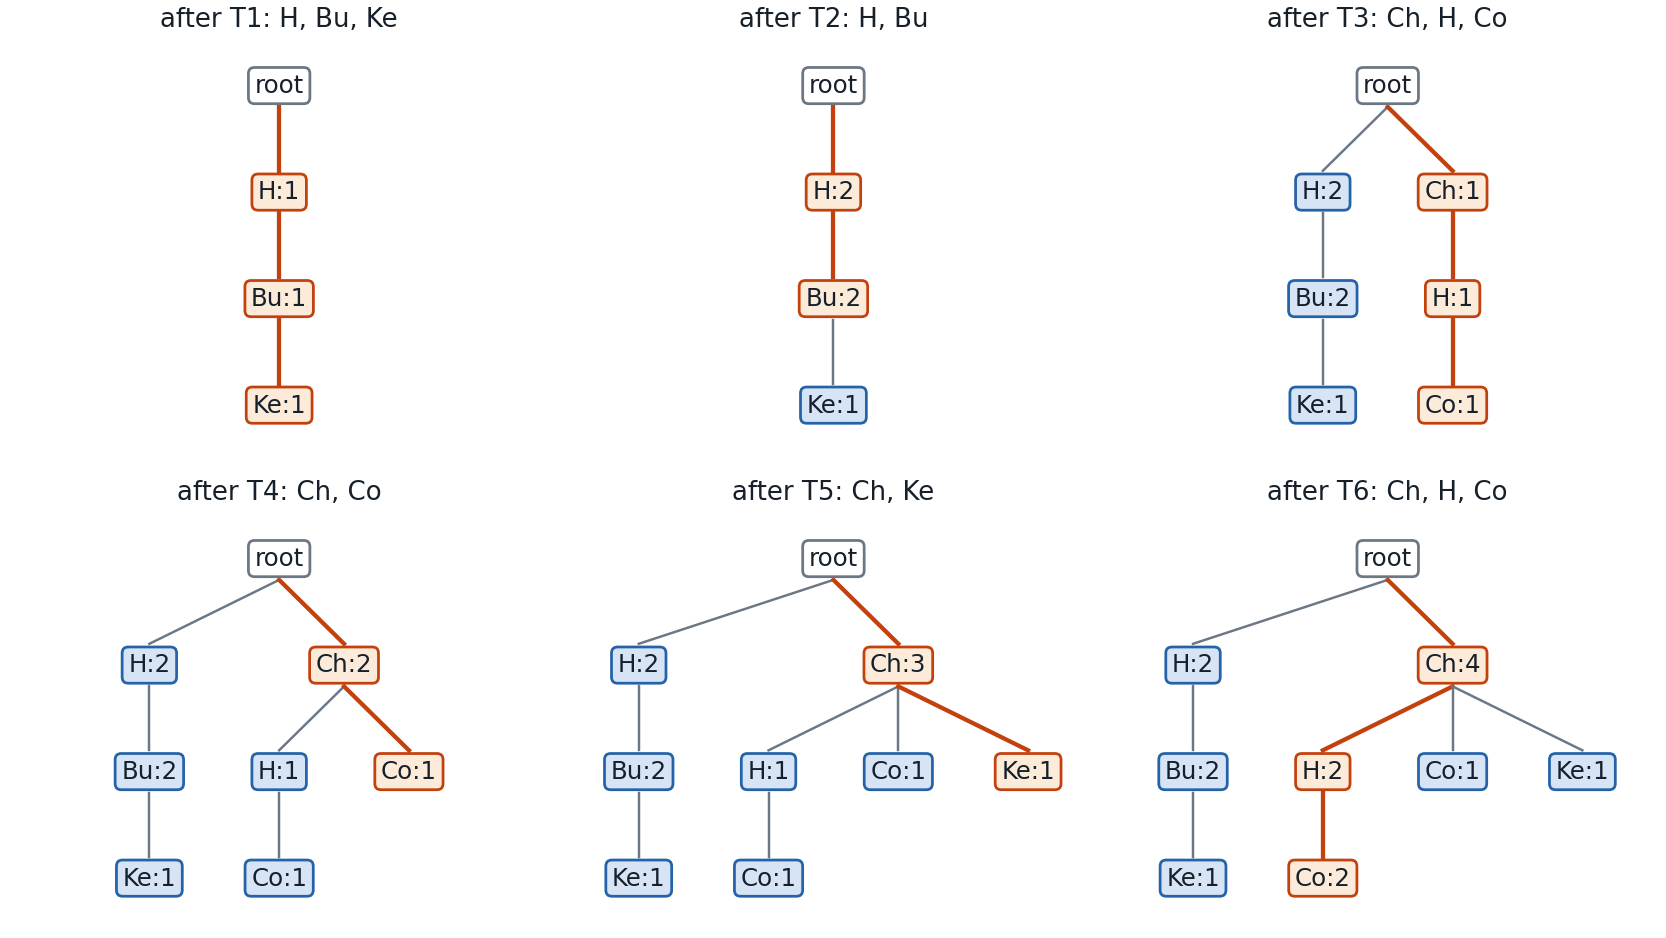
\includegraphics[width=0.84\textwidth]{figs/c4n_fp_78bh_steps.png}\hfill\mbox{}\par
{\color{sub}\footnotesize The path each transaction touches is in orange: a new branch where no
prefix is shared (T1, T3), incremented counts where it is (T2, T6). Drawn by \code{fpfig.py},
which rebuilds the tree from the transactions and checks every reordering and the final tree
against this page.}

\penalty0\vspace{3pt}
\lead{Mining, least-frequent item first}
\par
\begin{tabularx}{\textwidth}{@{}L{1.7cm}XL{6.0cm}@{}}
\toprule
\hrow \thead{Item} & \thead{Conditional pattern base} & \thead{Totals $\rightarrow$ patterns} \\
\midrule
Ketchup & \{H, Bu\}:1, \; \{Ch\}:1 & H:1, Bu:1, Ch:1 $\rightarrow$ \mk{all below 2, no pattern} \\
Buns    & \{H\}:2                  & H:2 $\rightarrow$ \{H, Bu\}:2 \\
Coke    & \{Ch, H\}:2, \; \{Ch\}:1 & Ch:3, H:2 $\rightarrow$ \{Ch,Co\}:3, \{H,Co\}:2,
                                     \textbf{\{Ch,H,Co\}:2} \\
HotDogs & \{\ \}:2, \; \{Ch\}:2    & Ch:2 $\rightarrow$ \{Ch, H\}:2 \\
Chips   & --- (root child)         & --- $\rightarrow$ \{Ch\}:4 \\
\bottomrule
\end{tabularx}

\lead{Frequent itemsets}
\begin{itemize}
  \item \textbf{1-itemsets}: Chips 4, HotDogs 4, Coke 3, Buns 2, Ketchup 2
  \item \textbf{2-itemsets}: \{Chips,Coke\} 3, \{Chips,HotDogs\} 2, \{HotDogs,Coke\} 2,
        \{HotDogs,Buns\} 2
  \item \textbf{3-itemsets}: \{Chips,HotDogs,Coke\} 2
  \item \mk{HotDogs has an empty prefix once} (it is a root child from T1/T2), which contributes
        nothing to its conditional base. Write the empty set rather than omitting the row.
\end{itemize}

\creamq{Problem 3.4}{\m{2+8}}
\begin{asked}{2074 Chaitra \textperiodcentered{} Q6 \textperiodcentered{} [2+8]}
How does FP growth approach overcomes the disadvantages of Apriori algorithm. For the
transaction data given in table generate FP-Tree.
\par\vspace{2pt}
\par
\begin{tabularx}{0.58\textwidth}{@{}L{3.0cm}X@{}}
\toprule
\hrow \thead{Transaction ID} & \thead{Item set} \\
T1 & Camera, Laptop, Pen drive \\
T2 & Laptop, Pen drive \\
T3 & Laptop, Mobile, Earphone \\
T4 & Earphone, Mobile \\
T5 & Camera, Earphone \\
T6 & Laptop, Mobile, Earphone \\
\bottomrule
\end{tabularx}
\end{asked}
{\color{sub}\footnotesize Min support is not printed; use 2. \gap Abbreviations:
E $=$ Earphone, L $=$ Laptop, Mo $=$ Mobile, Ca $=$ Camera, Pd $=$ Pen drive.}

\sbsr{0.53}{%
\lead{Step 1: counts and F-list}
\par
\begin{tabularx}{\linewidth}{@{}L{2.3cm}X L{1.0cm}L{0.9cm}@{}}
\toprule
\hrow \thead{Item} & \thead{In} & \thead{Count} & \thead{Keep} \\
\midrule
Earphone  & T3, T4, T5, T6 & 4 & \checkmark \\
Laptop    & T1, T2, T3, T6 & 4 & \checkmark \\
Mobile    & T3, T4, T6     & 3 & \checkmark \\
Camera    & T1, T5         & 2 & \checkmark \\
Pen drive & T1, T2         & 2 & \checkmark \\
\bottomrule
\end{tabularx}
\par\penalty0\vspace{1pt}
\textbf{F-list $=$ E(4), L(4), Mo(3), Ca(2), Pd(2)} \; --- \mk{all five are frequent}, and the
E/L tie at 4 is broken alphabetically.

\lead{Step 2: reorder each transaction by the F-list}
\par
\begin{tabularx}{\linewidth}{@{}L{0.7cm}L{3.4cm}X@{}}
\toprule
\hrow \thead{T} & \thead{As printed} & \thead{Reordered} \\
\midrule
T1 & Camera, Laptop, Pen drive & L, Ca, Pd \\
T2 & Laptop, Pen drive         & L, Pd \\
T3 & Laptop, Mobile, Earphone  & E, L, Mo \\
T4 & Earphone, Mobile          & E, Mo \\
T5 & Camera, Earphone          & E, Ca \\
T6 & Laptop, Mobile, Earphone  & E, L, Mo \\
\bottomrule
\end{tabularx}}{%
\lead{Step 3: insert them one at a time}
\par
\begin{tabularx}{\linewidth}{@{}L{0.7cm}X@{}}
\toprule
\hrow \thead{T} & \thead{Effect on the tree} \\
\midrule
T1 & new branch \texttt{L:1$\rightarrow$Ca:1$\rightarrow$Pd:1} \\
T2 & L:2, new child \texttt{Pd:1} under L \\
T3 & \mk{new root child} \texttt{E:1$\rightarrow$L:1$\rightarrow$Mo:1} \\
T4 & E:2, new child \texttt{Mo:1} under E \\
T5 & E:3, new child \texttt{Ca:1} under E \\
T6 & fully shared $\rightarrow$ E:4, L:2, Mo:2 \\
\bottomrule
\end{tabularx}
\begin{itemize}
  \item \mk{Two root children}: T1 and T2 hold no Earphone, so they cannot join the E prefix.
\end{itemize}}

\penalty0\vspace{2pt}
\lead{Final FP-tree}
\par\penalty0\vspace{1pt}
\begin{center}
\par
\begin{tikzpicture}[fptree, level 1/.style={sibling distance=62mm},
                    level 2/.style={sibling distance=20mm},
                    level 3/.style={sibling distance=18mm}, scale=0.82,
                    every node/.append style={transform shape}]
\node[fproot]{root}
  child { node{L:2}
    child { node{Ca:1} child { node{Pd:1} } }
    child { node{Pd:1} } }
  child { node{E:4}
    child { node{L:2} child { node{Mo:2} } }
    child { node{Mo:1} }
    child { node{Ca:1} } };
\end{tikzpicture}
\end{center}

\begin{itemize}
  \item \mk{Check}: L appears 4 times in $D$ and the tree shows 2 under the root plus 2 under E.
        \checkmark\ Do this for one item, it catches most construction errors.
  \item Mining it gives the key pattern \textbf{\{Earphone, Laptop, Mobile\}:2} (T3 and T6).
        The question only asks for the tree, so this is a bonus line.
\end{itemize}

\hr

%=======================================================================
\T{M4. Pattern evaluation: lift and correlation}

\lead{Method}
\[ lift(A,B) = \frac{P(A\cup B)}{P(A)\,P(B)} = \frac{conf(A\Rightarrow B)}{sup(B)}
   \qquad \chi^2 = \sum\frac{(obs-exp)^2}{exp} \]
\begin{itemize}
  \item $lift > 1$ positive $\cdot$ $=1$ independent $\cdot$ $<1$ negative.
\end{itemize}

\creamq{Problem 4.1}{\m{8}}
\begin{asked}{2070 Chaitra \textperiodcentered{} Q5 \textperiodcentered{} [8]}
Why is pattern evaluation important in association rule mining? Explain with example the
statistical based measures used for measuring interestingness of association rules.
\end{asked}
{\color{sub}\footnotesize The paper prints no data --- the example is yours to supply. The
standard \emph{game / video} contingency table below is the one every textbook uses. \added}

\lead{Given} 10,000 transactions: 6,000 contain \emph{game}, 7,500 contain \emph{video},
4,000 contain both.

\lead{Step 1: the support--confidence view says the rule is strong}
\begin{itemize}
  \item $sup(game \Rightarrow video) = 4000/10000 = \mathbf{40\%}$ \hfill (passes a 30\% threshold)
  \item $conf(game \Rightarrow video) = 4000/6000 = \mathbf{66.7\%}$ \hfill (passes a 60\% threshold)
\end{itemize}

\lead{Step 2: but look at the consequent alone}
\begin{itemize}
  \item $P(video) = 7500/10000 = \mathbf{75\%}$
  \item \mk{Buying a game DROPS the chance of buying a video from 75\% to 66.7\%.}
        The rule is actively misleading.
\end{itemize}

\lead{Step 3: lift catches it}
\[ lift = \frac{0.40}{0.60 \times 0.75} = \frac{0.40}{0.45} = \mathbf{0.89} < 1
   \ \rightarrow\ \text{negatively correlated} \]

\lead{Step 4: $\chi^2$ agrees}
\par
\begin{tabularx}{0.66\textwidth}{@{}L{2.2cm}XXL{1.6cm}@{}}
\toprule
\hrow & \thead{game} & \thead{$\overline{game}$} & \thead{row} \\
video & 4000 \emph{(4500)} & 3500 \emph{(3000)} & 7500 \\
$\overline{video}$ & 2000 \emph{(1500)} & 500 \emph{(1000)} & 2500 \\
col & 6000 & 4000 & 10,000 \\
\bottomrule
\end{tabularx}
\[ \chi^2 = \tfrac{500^2}{4500}+\tfrac{500^2}{3000}+\tfrac{500^2}{1500}+\tfrac{500^2}{1000}
   = 55.6+83.3+166.7+250 = \mathbf{555.6} \]
\begin{itemize}
  \item Large $\chi^2$ $\rightarrow$ correlated; observed (4000) $<$ expected (4500)
        $\rightarrow$ \textbf{negatively}.
\end{itemize}

\lead{Final answer}
\begin{itemize}
  \item \mk{Pattern evaluation matters because support and confidence alone certify rules that are
        false.} Add a correlation measure before reporting any rule.
  \item Mention that lift and $\chi^2$ are \textbf{not null-invariant}, so for sparse data prefer
        \textbf{all\_conf, max\_conf, Kulczynski or cosine}.
\end{itemize}

\hr

%=======================================================================
\T{M5. Subsequence enumeration}

\lead{Method}
\begin{itemize}
  \item A \textbf{$k$-subsequence} contains $k$ \emph{items} in total (not $k$ elements).
  \item Choose how many items to take from each element, keeping element order; a chosen element
        must be non-empty to remain in the sequence.
  \item \mk{Enumerate systematically} by the split $(a,b,c,d)$ of items taken per element,
        then remove duplicates.
\end{itemize}

\creamq{Problem 5.1}{\m{3}}
\begin{asked}{2076 Chaitra \textperiodcentered{} Q8 (a) \textperiodcentered{} [3]}
List all the 4-subsequences contained in the data sequence:
$\langle \{1,3\}\ \{2\}\ \{2,3\}\ \{4\} \rangle$
\end{asked}

\lead{Given} $e_1=\{1,3\}$, $e_2=\{2\}$, $e_3=\{2,3\}$, $e_4=\{4\}$; 6 items in total.

\sbs{%
\lead{What counts as a subsequence \mk{(get this right first)}}
\begin{itemize}
  \item Take a subset from each element, \mk{possibly empty}. Elements chosen empty simply
        disappear.
  \item \mk{Element order must be preserved}, and items from two different elements can never be
        merged into one element.
  \item \textbf{A $k$-subsequence has $k$ \emph{items} in total}, counted across all surviving
        elements. It is \mk{not} $k$ elements. This is the single most common misreading.
  \item So $\langle\{1,3\}\{2\}\rangle$ is a 3-subsequence, not a 2-subsequence.
\end{itemize}}{%
\lead{Why enumerate by splits}
\begin{itemize}
  \item A choice is fully described by \mk{how many items are taken from each element}, written
        $(a,b,c,d)$ for $e_1 \ldots e_4$.
  \item The bounds are the element sizes: $a\le2$, $b\le1$, $c\le2$, $d\le1$, and we need
        $a+b+c+d = 4$.
  \item For a fixed split the number of ways is a product of binomials,
        \mk{$\binom{2}{a}\binom{1}{b}\binom{2}{c}\binom{1}{d}$}, because the elements are chosen
        independently.
  \item \mk{Enumerating splits first guarantees nothing is missed}, which listing by hand does
        not. Then remove duplicates at the end.
\end{itemize}}

\penalty0\vspace{2pt}
\lead{Step 1: enumerate the item-count splits} $(a,b,c,d)$ with $a\le2, b\le1, c\le2, d\le1$, sum $=4$\par
\begin{tabularx}{0.9\textwidth}{@{}L{2.2cm}L{1.6cm}X@{}}
\toprule
\hrow \thead{$(a,b,c,d)$} & \thead{Ways} & \thead{Subsequences} \\
(2,1,1,0) & 2 & $\langle\{1,3\}\{2\}\{2\}\rangle$, $\langle\{1,3\}\{2\}\{3\}\rangle$ \\
(2,1,0,1) & 1 & $\langle\{1,3\}\{2\}\{4\}\rangle$ \\
(2,0,2,0) & 1 & $\langle\{1,3\}\{2,3\}\rangle$ \\
(2,0,1,1) & 2 & $\langle\{1,3\}\{2\}\{4\}\rangle$ \mk{(duplicate)}, $\langle\{1,3\}\{3\}\{4\}\rangle$ \\
(1,1,2,0) & 2 & $\langle\{1\}\{2\}\{2,3\}\rangle$, $\langle\{3\}\{2\}\{2,3\}\rangle$ \\
(1,1,1,1) & 4 & $\langle\{1\}\{2\}\{2\}\{4\}\rangle$, $\langle\{1\}\{2\}\{3\}\{4\}\rangle$,
                $\langle\{3\}\{2\}\{2\}\{4\}\rangle$, $\langle\{3\}\{2\}\{3\}\{4\}\rangle$ \\
(1,0,2,1) & 2 & $\langle\{1\}\{2,3\}\{4\}\rangle$, $\langle\{3\}\{2,3\}\{4\}\rangle$ \\
(0,1,2,1) & 1 & $\langle\{2\}\{2,3\}\{4\}\rangle$ \\
\bottomrule
\end{tabularx}

\lead{Step 2: check the count, then remove duplicates}
\begin{itemize}
  \item Ways per split: $2+1+1+2+2+4+2+1 = \mathbf{15}$ selections.
        \mk{Do this arithmetic} --- it is how you know no split was dropped.
  \item \mk{A duplicate appears when the same items can be taken from different elements.}
        Here $e_2 = \{2\}$ and $e_3 = \{2,3\}$ share the item 2, so
        $\langle\{1,3\}\{2\}\{4\}\rangle$ is produced twice: once as $(2,1,0,1)$ taking the 2 from
        $e_2$, once as $(2,0,1,1)$ taking it from $e_3$. \mk{Same sequence, so it counts once.}
  \item No other pair of splits can collide, because every other split keeps a different number
        of surviving elements or a different element content.
\end{itemize}

\lead{Final answer}
\begin{itemize}
  \item 15 selections $-$ 1 duplicate $\rightarrow$ \mk{\textbf{14 distinct 4-subsequences}}.
  \item \mk{The exam usually only wants ``at least four''} \yr{79 Bh}, so listing the first few from a
        clearly stated method is enough. \textbf{Show the method, not just the list.}
\end{itemize}

\creamq{Problem 5.2}{\m{3}}
\begin{asked}{2079 Bhadra \textperiodcentered{} Q6 (a) \textperiodcentered{} [3+3]}
How do you handle the categorical attributes in data mining process? Explain with example.
Generate the at least four subsequences from the given sequence:
$<\{2,3,5\}, \{6,7,8\}, \{9,1\}, \{7,4\}>$.
\end{asked}
\begin{itemize}
  \item Any order-preserving selection works. Four valid examples:
  \begin{itemize}
    \item $\langle\{2\}\{6\}\rangle$ \qquad $\langle\{3,5\}\{7\}\{9\}\rangle$
    \item $\langle\{2,3\}\{6,7\}\{1\}\{4\}\rangle$ \qquad $\langle\{5\}\{8\}\{9,1\}\{7\}\rangle$
  \end{itemize}
  \item \mk{Must hold}: element order preserved, and each chosen sub-element is a subset of the
        original element. \mk{Must not do}: reorder elements, or merge items from two elements
        into one.
\end{itemize}
%=======================================================================
\T{M6. Subgraph candidate generation by edge growing}

\lead{Method}
\begin{itemize}
  \item Two frequent subgraphs are joined only if they share a \textbf{common core}: the
        subgraph left when one edge is removed from each.
  \item \textbf{Edge growing} joins two $k$-edge graphs sharing a $(k-1)$-edge core and produces a
        \mk{$(k+1)$-edge candidate} $=$ core $+$ the edge unique to each parent.
  \item \textbf{Vertex growing} instead adds a vertex, and generates far more candidates.
        \mk{Edge growing is preferred for exactly that reason.}
  \item \mk{The trap, and the whole point of this question}: when the core carries
        \textbf{repeated vertex labels}, the two extra edges can be attached in more than one
        non-isomorphic way, so \mk{one join yields several candidates}. Enumerate them, do not
        assume there is one.
\end{itemize}

\creamq{Problem 6.1}{\m{3}}
\begin{asked}{2076 Chaitra \textperiodcentered{} Q8 (b) \textperiodcentered{} [3]}
Draw all candidate sub-graphs obtained from joining the pair of graphs shown below using
edge-growing method to expand the sub-graphs.
\par\penalty0\vspace{2pt}
\figC{pyq_subgraph_76ch.png}{0.52\textwidth}
\end{asked}

\sbs{%
\lead{Step 1: read the two parents}
\begin{itemize}
  \item Both are a \textbf{4-cycle of $a$ vertices} with two pendant vertices hanging off two
        \emph{adjacent} corners of that cycle.
  \item $G_1$: pendants are $b$ and $b$. \quad $G_2$: pendants are $b$ and $c$.
  \item Each has \textbf{6 vertices and 6 edges}, so $k = 6$.
\end{itemize}

\lead{Step 2: find the core}
\begin{itemize}
  \item Delete one edge from each so that what is left is the same graph:
        drop the second pendant edge from both.
  \item \mk{Core $=$ 4-cycle of $a$'s $+$ one pendant $b$}, 5 vertices and \textbf{5 edges}
        $= k-1$. \checkmark\ the graphs are joinable.
  \item Edge unique to $G_1$: $a - b$. \quad Edge unique to $G_2$: $a - c$.
\end{itemize}

\lead{Step 3: the candidate size}
\begin{itemize}
  \item Candidate $=$ core $+$ both unique edges $\rightarrow$ $5 + 2 = \mathbf{7}$ edges,
        7 vertices.
\end{itemize}}{%
\lead{Step 4: where can the two new edges attach?}
\begin{itemize}
  \item Call the core's pendant-carrying $a$ vertex $A_1$. In \emph{both} parents the second
        pendant sits on a cycle vertex \textbf{adjacent to $A_1$}, and $A_1$ has two neighbours
        in the cycle, $A_2$ and $A_4$.
  \item All four placements $(b,c)$ are legal: $(A_2,A_2)$, $(A_4,A_4)$, $(A_2,A_4)$, $(A_4,A_2)$.
  \item The core has a \mk{mirror symmetry swapping $A_2$ and $A_4$}, so these collapse to
        \textbf{two} non-isomorphic candidates:
  \begin{itemize}
    \item[] $(A_2,A_2)\cong(A_4,A_4)$ $\rightarrow$ \textbf{candidate I}
    \item[] $(A_2,A_4)\cong(A_4,A_2)$ $\rightarrow$ \textbf{candidate II}
  \end{itemize}
  \item \mk{This multiplicity comes entirely from the four $a$'s sharing one label.} Had the
        cycle been $a,b,c,d$ the join would have given a single candidate.
\end{itemize}}

\penalty0\vspace{3pt}
\lead{\mk{Final answer: 2 candidate sub-graphs}, each with 7 vertices and 7 edges}

\begin{center}
\par
\begin{tikzpicture}[gv/.style={circle,draw=ink,thick,inner sep=0.7pt,minimum size=13pt,
                               font=\footnotesize},
                    every path/.style={draw=ink,thick}, scale=0.95]
% ---------------- candidate I : both new pendants on the same corner
\begin{scope}
  \node[gv] (a1) at (1.1,1.1) {$a$};
  \node[gv] (a2) at (2.4,1.1) {$a$};
  \node[gv] (a3) at (2.4,0)   {$a$};
  \node[gv] (a4) at (1.1,0)   {$a$};
  \node[gv] (b0) at (0,1.1)   {$b$};
  \node[gv] (b1) at (0,0)     {$b$};
  \node[gv] (c1) at (1.1,-1.1){$c$};
  \draw (a1)--(a2) (a2)--(a3) (a3)--(a4) (a4)--(a1);
  \draw (b0)--(a1) (b1)--(a4) (c1)--(a4);
  \node[font=\footnotesize\bfseries,text=acc] at (1.2,-1.85) {Candidate I};
  \node[font=\scriptsize,text=sub,align=center] at (1.2,-2.35)
       {both new pendants\\on the same $a$};
\end{scope}
% ---------------- candidate II : new pendants on the two different neighbours
\begin{scope}[xshift=6.2cm]
  \node[gv] (B1) at (1.1,1.1) {$a$};
  \node[gv] (B2) at (2.4,1.1) {$a$};
  \node[gv] (B3) at (2.4,0)   {$a$};
  \node[gv] (B4) at (1.1,0)   {$a$};
  \node[gv] (C0) at (0,1.1)   {$b$};
  \node[gv] (C1) at (0,0)     {$b$};
  \node[gv] (C2) at (3.5,1.1) {$c$};
  \draw (B1)--(B2) (B2)--(B3) (B3)--(B4) (B4)--(B1);
  \draw (C0)--(B1) (C1)--(B4) (C2)--(B2);
  \node[font=\footnotesize\bfseries,text=acc] at (1.6,-1.85) {Candidate II};
  \node[font=\scriptsize,text=sub,align=center] at (1.6,-2.35)
       {new pendants on the two\\different neighbours of $A_1$};
\end{scope}
\end{tikzpicture}
\end{center}

\begin{itemize}
  \item \mk{Marking note}: the marks are for showing the \emph{core} and then arguing the
        placements. A single drawing with no core and no count of candidates scores badly even
        if the drawing itself is one of the two right answers.
  \item \mk{Cross-check}: every candidate must contain both parents as subgraphs, and must have
        exactly $k+1 = 7$ edges. Both do.
\end{itemize}
